%%%%%%%%%%%%%%%%%%%%%%%%%%%%%%%%%%%%%%%%%%%%%%%%%%%%%%%%%%%%%%%%%%%%%%
%
% Documento PRINCIPAL de Pedometria
% Newsletter da Sociedade Brasileira de Ciência do Solo
%
% Número 3, Março de 2014
% 
% Language: Latex
% 
%%%%%%%%%%%%%%%%%%%%%%%%%%%%%%%%%%%%%%%%%%%%%%%%%%%%%%%%%%%%%%%%%%%%%%

% PREÂMBULO
\documentclass[a4paper]{report}

% Língua e codificação
\usepackage[brazilian]{babel}
\usepackage[utf8]{inputenc}
\usepackage[T1]{fontenc}
%\usepackage[latin1]{inputenc}
%\DeclareUnicodeCharacter{00A0}{~}

% para boot
\usepackage{amssymb,amsmath}

% Nota: é preciso incluir o pacote amsmath antes do pacote PEDOMETRIAnews
% porque o último redefine o ambiente de equações
\usepackage{PEDOMETRIAnews}
\usepackage[round]{natbib}

% Figuras
\usepackage{graphicx} % evitar problemas com tamanho das figuras
\usepackage{wrapfig}

% para Sweave
\usepackage{listings}
\usepackage{Sweave}

% cor para verbatim (ambiente para código fonte)
\usepackage{color}
\let\oldv\verbatim
\let\oldendv\endverbatim
\def\verbatim{\par\setbox0\vbox\bgroup\oldv}
\def\endverbatim{\oldendv\egroup\fboxsep0pt \noindent\colorbox[gray]{0.8}{\usebox0}\par}

% definição de pedometria
\newcommand{\pedometria}{\textsc{PedometriA}}

% para tcltk-update
\usepackage{shortvrb}
%\usepackage{chapterbib}

\sloppy{}

% links
\usepackage{hyperref} % Deve ser o último pacote carregado
\hypersetup{colorlinks=true, citecolor=blue, linkcolor=blue, urlcolor=blue}

% DOCUMENTO
\begin{document}
 
% Edição da newsletter
\volume{3}
\volnumber{3}
\date{Março de 2014}
\titlepage

\begin{article}
   \title{Editorial}
\author{por Alessandro Samuel-Rosa}
\maketitle
\begin{wrapfigure}{l}{0.15\textwidth}
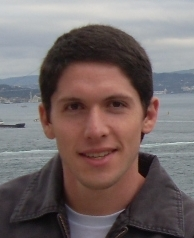
\includegraphics[width=0.15\textwidth]{figuras/foto-alessandro}
\end{wrapfigure}
O segundo número da \textit{Newsletter} da Comissão de Pedometria está cheio de novidades. A principal delas é a nova estrutura, muito mais bonita, graças à inestimável colaboração da comissão editorial do GRASS News, a newsletter do projeto \href{http://grass.osgeo.org/newsletter/}{GRASS}. Após contato com Martin Wegmann \email{wegmann@biozentrum.uni-wuerzburg.de}, editor-chefe do GRASS News, e Dylan Beaudette \email{debeaudette@ucdavis.edu}, administrador da página da web do GRASS News, formos gentilmente autorizados a usar o arquivo de estilo \texttt{GRASSnews.sty}, originalmente derivado do arquivo de estilo \texttt{Rnews.sty}, usado pela equipe do projeto \R{} para produção da sua newsletter. O agora arquivo de estilo da \textit{Newsletter} da Comissão de Pedometria da SBCS, \texttt{PEDOMETRIAnews.sty}, está disponível para baixar \href{http://goo.gl/OBWF3s}{clicando aqui}. É por meio do arquivo de estilo \texttt{PEDOMETRIAnews.sty} que a \textit{Newsletter} fica com a cara que ela tem hoje. Mais informações sobre o uso de \LaTeX{} para a produção de documentos técnico-científicos podem ser encontradas no site da \href{http://www.elsevier.com/author-schemas/preparing-documents-with-tex}{Elsevier}.\\
A evolução da \textit{Newsletter} em seu segundo número acompanha a evolução da pedometria no Brasil, claramente evidenciada pelo volume de trabalhos publicados no Congresso Brasileiro de Ciência do Solo (CBCS), em Florianópolis, há alguns meses atrás. Somam-se aí os espaços destinados mesas de discussão constituídas por importantes pesquisadores da pedometria nacional e internacional. O espaço destinado pela Comissão Organizadora do CBCS mostra que a comunidade científica nacional, assim como já ocorre há mais de uma década em outros países, está muito interessada nas contribuições da mais nova disciplina da ciência do solo. Uma disciplina que exige, como mostram os artigos que seguem, uma abordagem mais do que multidisciplinar ou interdisciplinar. Uma disciplina que exige uma abordagem \href{http://www.fisica-interessante.com/files/artigo-transdisciplinaridade.pdf}{transdisciplinar}, forçando-nos a transpor os limites das disciplinas tradicionais da ciência do solo e mergulhar em um universo de novas maneiras de 
encarar velhos problemas.
%%% Local Variables: 
%%% mode: latex
%%% TeX-master: documento-principal.tex
%%% End: 


\end{article}

\begin{article}
   \title{Suscetibilidade Magnética nos Solos Tropicais}
\subtitle{Uma Alternativa Promissora}
\author{por Diego Silva Siqueira e José Marques Jr.}
\maketitle

\section{Suscetibilidade magnética: alternativa para aquisição indireta de informações detalhadas do solo e seus atributos}
\label{sec:1}

A falta de informações detalhadas sobre os recursos do solo é um dos fatores limitantes para o crescimento de diferentes áreas do conhecimento e setores produtivos. Apesar de informações detalhadas dos atributos dos solos serem escassas em território brasileiro, em países como China \citep{liu:2013} e EUA \citep{franze:2006} já são utilizadas nos planejamentos agrícolas e urbanos. Em alguns países da Europa informações da distribuição espacial dos atributos do solo auxiliam na avaliação do impacto da política agrícola em diferentes níveis de detalhe \citep{vandelden:2010}.

\begin{wrapfigure}{l}{0.15\textwidth}
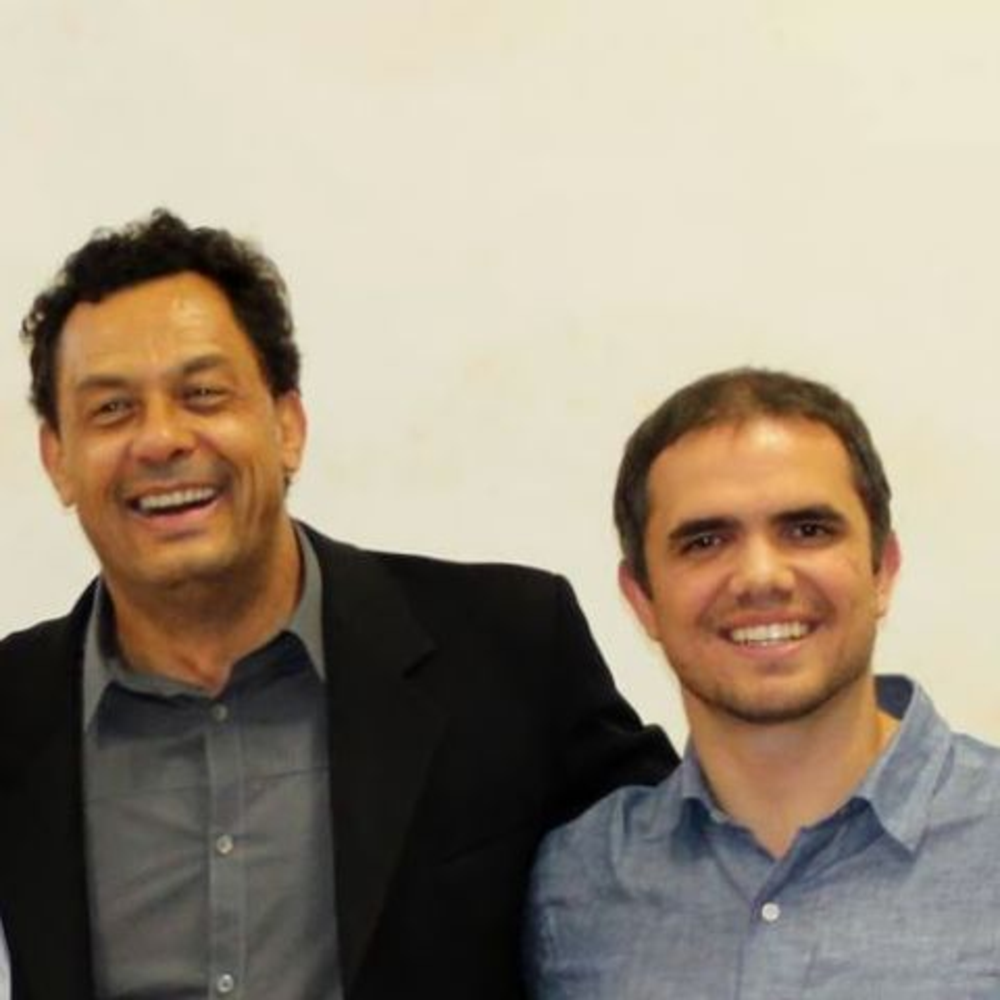
\includegraphics[width=0.15\textwidth]{figuras/foto-diego-junior}
\end{wrapfigure}

Frente às urgências e problemas relacionados à elaboração de um inventário de solos, a caracterização de atributos, pode ser uma alternativa para atender a demanda atual. Essa foi uma das soluções apontadas pelo Painel Técnico Intergovernamental sobre Solos (ITPS, da sigla em inglês) coordenado pela Organização das Nações Unidas para Alimentação e Agricultura (FAO), cujo objetivo é fornecer auxílio técnico e científico em assuntos globais sobre solos e seus atributos, para instituições mundiais ou regionais. Existe, portanto, um alinhamento de propostas sobre o solo e seus atributos para segurança alimentar e a sustentabilidade do planeta.




Porém, para atender a estes e outros objetivos, dois aspectos são fundamentais: - escolha do atributo, que deve ser sensível às variações dos fatores e processo de formação do solo (ex. óxidos de ferro) \citep{camargo:2013}; - ferramentas eficientes para caracterizar a variabilidade destes atributos de maneira precisa e, a baixo custo, viabilizando a caracterização detalhada da variabilidade para grandes áreas. Nesse sentido, destacam-se os avanços tecnológicos relacionados à aquisição de informações sobre os solos utilizando a condutividade elétrica \citep{brennin:2008}, suscetibilidade magnética (SM) \citep{grimley-vepraskas:2000} e espectroscopia de reflectância difusa (ERD) \citep{torrent-barron:1993}.




A condutividade elétrica foi originalmente desenvolvida para regiões temperadas com baixa expressão dos óxidos de ferro. Autores \citep{wu:2008} relatam que essa técnica sofre alterações em regiões com elevada presença de óxidos. Por este motivo, nos solos tropicais, resultados de pesquisas indicam que a SM é uma boa alternativa para identificação de áreas com diferentes padrões de variabilidade \citep{camargo:2013}, bem como na quantificação indireta de atributos físicos, químicos e mineralógicos em áreas com baixo ($Fe_{2}O_{3}<40\text{ g kg}^{-1}$) \citep{siqueira:2010} e alto teor de ferro ($Fe_{2}O_{3}>180\text{ g kg}^{-1}$) \citep{peluco:2013}.




\section{Magnetismo e suscetibilidade magnética: diferença, origem e evolução na Ciência do Solo}
\label{sec:2}




Enquanto o magnetismo está relacionado ao fenômeno de atração ou repulsão, a SM está relacionada com capacidade de um material em magnetizar-se. Mas como os materiais naturais, a exemplo das rochas e minerais se magnetizam?




As rochas podem se magnetizar de diferentes maneiras, a mais comum, é chamada de magnetização termo-remanescente \citep{press:2006}. Porém, antes de esclarecer sobre o processo de magnetização, é preciso conhecer alguns conceitos mineralógicos, como cela unitária. A cela unitária é a menor parte dos minerais presentes nas rochas e nos solos. No centro da cela unitária dos óxidos de ferro, por exemplo, o átomo mais encontrado é o ferro. A magnetização, está relacionada com os elétrons deste átomo. Para saber um pouco mais sobre o assunto "Óxidos de Ferro: Pedoindicadores Ambientais", bem como visualizar figuras e esquemas,recomendamos algumas apresentações do Grupo de Pesquisa CSME (\href{http://www.acervodigital.unesp.br/handle/123456789/40434}{Caracterização do Solo para fins de Manejo Específico}). Retomando, na magnetização termo-remanescente, os elétrons da cela unitária dos minerais magnéticos presentes nas rochas ígneas, orientam-se na direção do campo magnético da Terra na época em que a cela unitária foi formada. Dessa maneira, os minerais ``gravam'' a magnetização do local e da época de formação da rocha. Por este motivo, diz-se que os minerais com capacidade magnética armazenam arquivos naturais contendo registros dos fatores de formação do solo \citep{maher-thompson:1999}, sendo considerados como pedoindicadores. Os minerais também podem adquirir magnetizações posteriores a sua formação, em virtude de processos físicos e químicos. Esse tipo de magnetização é chamado de magnetização remanescente secundária \citep{teixeira:2009}. Para saber um pouco mais sobre magnetismo dos minerais acesse o link \url{http://www.on.br/ead_2012/pdf/modulo2/4_magnetismo_das_rochas.pdf}.




O alinhamento dos elétrons da cela unitária dos minerais, mencionado anteriormente, está relacionado com o spin, que nada mais é do que o movimento de rotação do elétron em um sentido. Quando os elétrons rotacionam em um mesmo sentido, diz-se que há um alinhamento. Conforme descoberto por Hans Christian Orsted em 1820, as correntes elétricas podem criar campos magnéticos. Assim, a movimentação dos elétrons da cela unitária dos minerais, na estrutura cristalina (conjunto de celas unitárias), gera uma microcorrente elétrica, que por sua vez gera um campo magnético. A facilidade com que os elétrons têm de rotacionarem no mesmo sentido (spins pareados), faz com que o campo magnético produzido pelo mineral seja mais forte. Além da distribuição dos elétrons nos subníveis de energia, a direção de cristalização da rede cristalográfica do mineral também interfere em sua SM. Este efeito é conhecido como anisotropia magnética (Figura \ref{fig:figura1}).




\begin{figure*}[tb!]
\begin{minipage}[t]{1\linewidth}
\begin{center}
   \includegraphics[width=\textwidth]{figuras/figura-diego-junior}
   \caption{Diagrama da organização de elétrons do elemento ferro nas celas unitárias do mineral e tipos de suscetibilidade magnética proveniente da rotação dos elétrons (a), intervalo de suscetibilidade magnética para óxidos de ferro puros e rochas (b) (Modificado de DEARING, 1994), variação da suscetibilidade magnética em função da forma e do tamanho do mineral (c) (Modificado de \url{http://www.irm.umn.edu/hg2m/hg2m_c/Image18.gif}, Universidade de Minnesota, Colégio de Ciência e Engenharia) (Extraído de \cite{siqueira:2013})
   \label{fig:figura1}}
\end{center}
\end{minipage}
\end{figure*}




Portanto, a SM de um mineral está relacionada com a rotação dos elétrons da cela unitária dos minerais, presentes na rocha ou no solo \citep{craik:1995}. São considerados 5 tipos básicos de comportamento magnético: diamagnetismo, paramagnetismo, ferromagnetismo, ferrimagnetismo e antiferromagnetismo. Nos minerais diamagnéticos, o número de spins alinhados numa direção é igual ao número de spins na direção oposta, logo os campos magnéticos anulam-se (Exemplo: quartzo). Nos minerais paramagnéticos as camadas eletrônicas estão incompletas. A presença de um campo magnético externo faz com que os spins se alinhem (elétrons giram no mesmo sentido), e mesmo após a retirada do campo magnético, alguns spins permanecem alinhados (Exemplo: olivina). Os minerais ferromagnéticos são um caso especial de paramagnetismo. Após a retirada do campo magnético os spins permanecem alinhados, fazendo com que o mineral possua um grande valor de magnetização remanescente (Exemplo: ferro e cobalto). Nos minerais ferrimagnéticos, os spins não estão emparelhados, assim prevalece a campo magnético resultante do maior número de spins no mesmo sentido (Exemplo: magnetita). Os minerais antiferromagnéticos não apresentam propriedades magnéticas.




Uma situação importante a ser relatada é referente à neosíntese de minerais, especialmente os óxidos de ferro. Quando um ambiente oxídico passa para ambiente redutor, ocorre uma alteração na neosíntese dos minerais, especialmente dos óxidos de ferro. No caso específico dos óxidos, pode ocorrer recristalização dos minerais e o ferro do núcleo da cela unitária, passa de seu estado oxidado ($Fe^{3+}$) para reduzido ($Fe^{2+}$). Com o processo de oxiredução, há nova redistribuição dos elétrons do átomo nas camadas de energia. A nova configuração eletrônica dos elétrons faz com que o número de spins rotacionando em sentidos opostos, seja mais equilibrada, diminuindo o valor da suscetibilidade magnética.




Muitas vezes a SM é confundida com atração magnética. A atração magnética foi utilizada como ferramenta auxiliar de campo nos primeiros levantamentos de solos do Estado de São Paulo na década de 1960 e 1970, para distinguir solos originados de rochas máficas de outros materiais de origem \citep{resende:1988}.




Nos solos originados de rochas máficas (ricos em magnetita e maghemita), quando um ímã qualquer é aproximado da superfície do solo, há atração entre suas partículas e o ímã, e o solo prende-se ao ímã. Portanto, a atração magnética pode ser interpretada como ferramenta qualitativa. No campo, os mapeadores notaram que, mesmo tratando-se de um solo originado de rocha máfica, havia diferentes intensidades de atração magnética. Em alguns locais, a superfície do ímã ficava mais recoberta por partículas de solo e, em outros locais, menos recoberta. Isso inspirou a aplicação da atração magnética como ferramenta quantitativa e estudos sobre a SM.




Porém, devido à dificuldade de reprodução dos resultados e à baixa exatidão entre os laboratórios para expressar as diferentes interações magnéticas das amostras de solo, a técnica caiu em desuso \citep{resende:1988}. Com os avanços dos sensores e de técnicas alternativas na avaliação da interação magnética \citep{carneiro:2003}, o uso da SM como ferramenta auxiliar na caracterização quantitativa da variabilidade de campo \citep{santos:2013} ganha novas expectativas.




Um dos equipamentos mais utilizados para avaliação da SM é o sensor da Bartington MS2, acoplado ao sensor Bartington MS2B. A avaliação pode ser feita no campo, em laboratório, em amostras de terra fina seca ao ar (TFSA) ou fração argila, silte e areia. Para aplicações em estudos de pedometria, com foco no desenvolvimento de funções de pedotransferência para quantificação, recomenda-se que sejam feitas avaliações em baixa frequência (0,47 kHz) \citep{dearing:1994}. Segundo estes autores, as medições de dupla frequência (alta – 4,7 kHz e baixa) devem ser utilizadas em estudo de caráter qualitativo para indicar a presença de minerais magnéticos de domínio simples, múltiplos e anisotropia magnética. Uma alternativa prática e barata para avaliação da SM é a utilização de uma balança analítica. Os resultados de SM, obtidos pela adaptação da balança, tiveram boa correlação ($R^{2}=0,942;\,P<0,01$) com os resultados obtidos pelo sensor da Bartington \citep{siqueira:2010}.




No sensoriamento remoto, o magnetismo e SM são utilizados rotineiramente como ferramenta, no detalhamento do mapa geológico \citep{ruy:2006} e recentemente no desenvolvimento de assinaturas geomagnéticas, para estudos detalhados sobre os solos da China \citep{xia:2007}. A vantagem em se utilizar informações geofísicas, está relacionada ao seu potencial para descrever processos de formação do solo, os quais dificilmente alteram-se em curto prazo por intermédio de ações antrópicas. A mineralogia do solo é um dos principais indicadores da variação destes processos pedogenéticos \citep{camargo:2013}. Como a SM é produto da variação dos minerais presentes do solo \citep{siqueira:2013}, podemos inferir que o mapa da SM expressa o mapa dos processos pedogenéticos do solo.




As aplicações do conhecimento sobre geofísica, especificamente do magnetismo, podem ser associadas à habilidade das áreas em explorar a multidisciplinaridade. Fazendo uma comparação das publicações com o termo ``\textit{magnetism}'', na base referencial multidisciplinar, Web of Science, entre as áreas Agronomia e Mineralogia, versos Ciências Ambientais e Ecologia, nota-se que, nas áreas Agronomia e Mineralogia, não houve aumento no número de publicações em 2013 (5 publicações) em comparação ao ano de 1997 (5 publicações). Em contra partida, na área de Ciências Ambientais e Ecologia, houve um aumento de 433\%, de 2013 (16 publicações) em comparação ao ano de 1997 (3 publicações). Este fato exemplifica a importância da multidisciplinaridade e corrobora relatos de pesquisadores brasileiros, a exemplo \cite{vidal-torrado:2005}, e estrangeiros, a exemplo \cite{grunwald:2011}, sobre a formação e educação do moderno cientista do solo, cuja reflexão é ``\textit{O quão multidisciplinar devemos ser frente aos desafios}?''.




\begin{footnotesize}
\begin{thebibliography}{99}




\bibitem[Brenning et~al.(2008)]{brennin:2008}
Brenning, A., Koszinski, S., Sommer, M. (2008)
\newblock Geostatistical homogenization of soil conductivity across field boundaries.
\newblock {\em Geoderma} 143: 254-260.




\bibitem[Camargo et~al.(2010)]{camargo:2010}
Camargo, L. A., Marques Jr., J., Pereira, G. T. (2010)
\newblock Spatial variability of physical attributes of an Alfisol under different hillslope curvatures.
\newblock {\em Revista Brasileira de Ciência do Solo} 34: 617-630.




\bibitem[Camargo(2013)]{camargo:2013}
Camargo, L. A. (2013)
\newblock Mineralogia da argila por difração de raios x e espectroscopia de reflectância difusa em Latossolos sob diferentes superfícies geomórficas.
\newblock {\em Tese (Doutorado) – Faculdade de Ciências Agrárias e Veterinárias, Universidade Estadual Paulista, Jaboticabal} 2013.




\bibitem[Carneiro et~al.(2003)]{carneiro:2003}
Carneiro, A. A. O., Touso, A. T., Baffa, O. (2003)
\newblock Avaliação da suscetibilidade magnética usando uma balança analítica.
\newblock {\em Química Nova} 26: 952-956.




\bibitem[Craik(1995)]{craik:1995}
Craik, D. (1995)
\newblock Magnetism, Principles and Aplications.
\newblock {\em John Wiley and Sons} p.1-459.




\bibitem[Dearing(1994)]{dearing:1994}
Dearing, J.A. (1994)
\newblock Environmental magnetic susceptibility. Using the Bartington MS2 system.
\newblock {\em England: British Library} 104 p. Disponível em: \url{http://gmw.com/magnetic\_properties/pdf/Om0409\%20J\_Dearing\_Handbook_iss7.pdf}.




\bibitem[Franze et~al.(2006)]{franze:2006}
Franzen, D. W., Nanna, T., Norvell, W. A. (2006)
\newblock A Survey of Soil Attributes in North Dakota by Landscape Position.
\newblock {\em Agronomy Journal} 98: 1015-1022.




\bibitem[Grimley e Vepraskas(2000)]{grimley-vepraskas:2000}
Grimley, D. A., Vepraskas, M. J. (2000)
\newblock Magnetic susceptibility for use in delineating hydric soils.
\newblock {\em Soil Science Society American Journal} 64: 2174-2180.




\bibitem[Grunwald et~al.(2011)]{grunwald:2011}
Grunwald, S., Thompson, J. A., Boettinger, J. L. (2011)
\newblock Digital Soil Mapping and Modeling at Continental Scales: Finding Solutions for Global Issues.
\newblock {\em Soil Science Society American Journal} 75: 1201-1213.




\bibitem[Liu et~al.(2013)]{liu:2013}
Liu, Y., Lv, J., Zhang, B., Bi, J. (2013)
\newblock Spatial multi-scale variability of soil nutrients in relation to environmental factors in a typical agricultural region, Eastern China.
\newblock {\em Science of the Total Environment} p. 108-119.




\bibitem[Maher e Thompson(1999)]{maher-thompson:1999}
Maher, B. A., Thompson, R. (1999)
\newblock Palaeomonsoons I: the magnetic record of palaeoclimate in the terrestrial loess and palaeosol sequences, in quaternary climates, environments and magnetism.
\newblock {\em Cambridge: University Press} p. 81–125.




\bibitem[Peluco et~al.(2013)]{peluco:2013}
Peluco, R. G., Marques Jr., Siqueira, D. S., Pereira, G. T., Barbosa, R. S., Teixeira, D. B., Adame, C. R., Cortez, L. A. (2013)
\newblock Suscetibilidade magnética do solo e estimação da capacidade de suporte à aplicação de vinhaça.
\newblock {\em Pesquisa Agropecuária Brasileira} 48:661-672.




\bibitem[Press et~al.(2006)]{press:2006}
Press, F., Siever, R., Grotzinger, J., Jordan, T. H. (2006)
\newblock Para entender a Terra. 4ª edição. Versão traduzida
\newblock {\em Bookman} p. 656.




\bibitem[Resende et~al.(1988)]{resende:1988}
Resende, M., Santana, D. P., Rezende, S. B. (1988)
\newblock Susceptibilidade magnética em Latossolo do Sudeste e Sul do Brasil.
\newblock {\em In: REUNIÃO DE CLASSIFICAÇÃO, CORRELAÇÃO DE SOLOS E INTERPRETAÇÃO DE APTIDÃO AGRÍCOLA, Rio de Janeiro, EMBRAPA-SNLCS/SBCS} p 233–258.




\bibitem[Ruy et~al.(2006)]{ruy:2006}
Ruy, A. C., Silva, A. M., Toledo, C. L. B.,Souza Filho, C. R. (2006)
\newblock Uso de dados aerogeofísicos de alta densidade para mapeamento geológico em terrenos altamente intemperizados: o estudo de caso da Região de Cláudio, porção Sul do Cráton São Francisco.
\newblock {\em Revista Brasileira de Geofísica} 24:535-546.




\bibitem[Santos et~al.(2013)]{santos:2013}
Santos, H. L., Marques Jr., J., Matias, S. S. R., Siqueira, D. S., Pereira, G. T. (2013)
\newblock Erosion factors and magnetic susceptibility in differet compartments of a slope in Gilbués-PI, Brazil.
\newblock {\em Engenharia Agrícola} 33:64-74.




\bibitem[Siqueira et~al.(2010)]{siqueira:2010}
Siqueira, D. S., Marques Jr., J., Matias, S. S. R., Barrón, V., Torrent, J., Baffa, O., Oliveira, L. C.  (2010)
\newblock Correlation of properties of Brazilian Haplustalfs with magnetic susceptibility measurements.
\newblock {\em Soil, Use and Management} 26:425-431.




\bibitem[Siqueira(2013)]{siqueira:2013}
Siqueira, D. S. (2013)
\newblock Mapeamento detalhado e planejamento amostral para Latossolos utilizando suscetibilidade magnética e cor no contexto da relação solo-paisagem.
\newblock {\em Tese (Doutorado) – Faculdade de Ciências Agrárias e Veterinárias, Universidade Estadual Paulista, Jaboticabal} 2013.




\bibitem[Teixeira et~al.(2009)]{teixeira:2009}
Teixeira, W., Toledo, M. C. M. De, Fairchild, T. R., Taioli, F. (2009)
\newblock Decifrando a Terra.São Paulo.
\newblock {\em Oficina de Textos} p.557.




\bibitem[Torrent e Barrón(1993)]{torrent-barron:1993}
Torrent, J., Barrón, V. (1993)
\newblock Laboratory measurements of soil color: theory and practice
\newblock {\em In: BIGHAM, J. M., CIOLKOSZ, E. J. (Ed) Soil Color. Soil Science Society of America, Special Publication} p. 21-33.




\bibitem[Van Delden et~al.(2010)]{vandelden:2010}
Van Delden, H., Stuczynski, T., Ciaian, P., Paracchini, M. L., Hurkens, J., Lopatka, A., Shi, Y., Gomez Prieto, O., Calvo, S., Van Vliet, J., Vanhout, R. (2010)
\newblock Integrated assessment of agricultural policies with dynamic land use change modelling.
\newblock {\em Ecological Modelling} 221:2153–2166.




\bibitem[Vidal-Torrado et~al.(2005)]{vidal-torrado:2005}
Vidal-Torrado, P., Lepsch, I. F., Castro, S. S. (2005)
\newblock Laboratory measurements of soil color: theory and practice
\newblock {\em In: P. Vidal-Torrado, Luiz R. Ferraciu, M. Cooper, Elke J. Cardoso, Luiz I. Prochonow. (Org.). Tópicos em Ciência do Solo. Viçosa: Sociedade Brasileira de Ciência do Solo} 4:145-192.




\bibitem[Wu et~al.(2008)]{wu:2008}
Wu,Y.; Slater, L.;  Versteeg, R.;  Labrecque, D. (2008)
\newblock A comparison of the low frequency electrical signatures of iron oxide versus calcite precipitation in granular zero valent iron columns.
\newblock {\em Journal of Contaminant Hydrology} 95:154–167.




\bibitem[Xia et~al.(2007)]{xia:2007}
Xia, D., Jin, M., Liu X., Chen F., Ma J., Zhao H., Wang X., Wei H. (2007)
\newblock A preliminary study on the magnetic signatures of modern soil in Central Asia.
\newblock {\em Frontiers of Earth Science} 1:275–283.

\end{thebibliography}
\end{footnotesize}

\address{Diego Silva Siqueira\\
  \begin{footnotesize}
    UNESP Câmpus de Jaboticabal - Grupo de Pesquisa CSME\\
    \url{http://lattes.cnpq.br/8836609544198735}\\
    \email{diego\_silvasiqueira@yahoo.com.br}
  \end{footnotesize}
}\\
\vskip
\address{José Marques Jr.\\
  \begin{footnotesize}
    UNESP Câmpus de Jaboticabal - Grupo de Pesquisa CSME\\
    \url{http://lattes.cnpq.br/5425582467938015}\\
    \email{marques@fcav.unesp.br}
  \end{footnotesize}
}
%%% Local Variables:
%%% mode: latex
%%% TeX-master: 3rd-edition.tex
%%% End:
\end{article}

\newpage

\begin{article}
   \title{Entrevista}
\subtitle{com Ricardo Bergamo Schenato}
\maketitle
\begin{wrapfigure}{l}{0.15\textwidth}
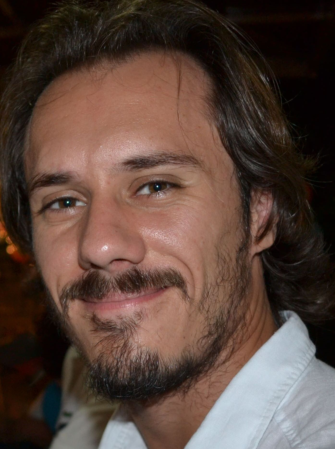
\includegraphics[width=0.15\textwidth]{figuras/foto-ricardo}
\end{wrapfigure}








Nesta edição de \pedometria, entrevistamos o Professor Doutor Ricardo Bergamo Schenato para falar um pouco sobre a Pedometria e a Modelagem Ambiental, suas potencialidades, dificuldades e perspectivas futuras no Brasil. O Dr. Ricardo atualmente é docente no Departamento de Solos - Setor de Gênese, Morfologia e Classificação de Solos da Universidade Federal de Santa Maria (UFSM). Sua formação pós ensino médio foi realizada na UFSM, onde cursou Agronomia e o mestrado em Ciência do Solo na área de Química do solo. Fez doutorado em Ciência do solo na Universidade Federal do Rio Grande do Sul (UFRGS). Sua tese contemplou temas relacionados a modelagem e fluxos de gases de efeito estufa no Estado do RS.
\\
\textbf{Pedometria} - O que levou você a se interessar e estudar temas relacionados a modelagem ambiental e em especial propriedades do solo?\\
\\
\textbf{Ricardo} - Na iniciação científica meu primeiro contato com a espacialização de propriedades e atributos de solo ocorreu quando trabalhei com a temática de agricultura de precisão, onde experimentei todas as fases da pesquisa. Nesta época comecei a interessar-me nas questões ambientais que envolviam o solo por ocasião da leitura de textos sobre qualidade do solo e por constatar que a maioria da pesquisa estava focada na melhoria ou conservação da capacidade produtiva em detrimento de uma compreensão global do sistema. Ainda na graduação, o interesse crescente na otimização dos recursos empregados na produção primária determinaram a escolha por estudar a transferência de elementos na paisagem, tornando-se o objeto de minha dissertação de mestrado. O interesse pela modelagem, em um sentido amplo, deveu-se às potencialidade que suas ferramentas oferecem para a pesquisa ambiental, podendo-se citar a capacidade de simular condições pretéritas e futuras, avaliar variáveis que seriam de difícil mensuração a campo, elaborar cenários complexos, extrapolar resultados no tempo e no espaço, auxiliar no planejamento da pesquisa empírica, entre outros.\\
\\
\textbf{Pedometria} - Quais são os projetos de pesquisa que você está desenvolvendo relacionados a modelagem ambiental e espacialização de propriedades do solos?\\
\\
\textbf{Ricardo} - Em novembro de 2013 ingressei como docente da UFSM, portanto, devido à entrada recente, estou readequando minhas linhas de pesquisa com o intuito de colaborar mais eficientemente com os pesquisadores do Departamento de Solos. A Pedometria será a principal linha de pesquisa, especialmente como subsídio ao Mapeamento Digital do Solo (MDS). O foco inicial será na avaliação de técnicas para determinar a distribuição espacial de classes e atributos do solo. A abrangência das aplicações da Pedometria, aliada ao caráter incipiente desta área quando comparada a outras da Ciência do Solo, resultam em uma grande possibilidade de interação, de tal forma que projetos com outras áreas do conhecimento certamente serão desenvolvidos. Além disso, pretendo dar continuidade e ampliar a pesquisa que desenvolvi na minha tese \citep{Schenato:2013}, visando a modelagem dos ciclos de C e N no solo e seu efeito na emissão de gases de efeito estufa, bem como implementar a espacialização dos resultados já obtidos. O objetivo principal desta linha é estimar os impactos, positivos e negativos, da atividade agropecuária e auxiliar no uso racional dos recursos.\\
\\
\textbf{Pedometria} - Qual sua opinião a respeito do cenário atual sobre as pesquisas em modelagem ambiental e predição de propriedades do solo no Brasil?\\
\\
\textbf{Ricardo} - A adesão dos pesquisadores em solos brasileiros a estes temas é relativamente recente, tanto que grande parte da produção científica nacional está concentrada especialmente na última década. Esta observação também mostra que existe um número crescente de profissionais publicando em ambos os assuntos, refletindo a importância destes e indicando um fortalecimento dos grupos de pesquisa. Os custos baixos e a facilidade de obtenção de dados de sensores remotos são fatores que propiciaram o aumento da sua utilização para a determinação de atributos do terreno como declividade, elevação, aspecto, plano de curvatura, radiação solar, índices topográficos, índice de convergência, entre outros, abrindo um campo importante para trabalhos que enfoquem a implicação destes atributos na dinâmica de formação e evolução do solo e da paisagem. A prevalência na utilização tanto da modelagem do terreno como na predição de propriedades do solo está voltada ao MDS, o que pode ser justificado pela lacuna existente no nosso país no tocante ao conhecimento mais detalhado das classes de solo e ao aumento da demanda por informações mais detalhadas como subsídio para aplicações práticas.  O planejamento de projetos agrícolas, a adequação do uso do solo urbano e a implementação de atividades de recuperação ambiental são apenas alguns exemplos que necessitam da definição adequada da classe e/ou de propriedades do solo e estas informações nem sempre estão disponíveis ou a escala não é adequada. Nestes casos a predição de propriedades pode facilitar a obtenção dos dados e baratear o custo dos projetos, considerando que o levantamento e a determinação clássica tendem a ser mais onerosos e demorados. A frequência na aplicação de funções de pedotransferência pelos pesquisadores brasileiros também merece destaque. A abrangência das informações que podem ser geradas e a disseminação do uso dessas funções tem um potencial muito grande, podendo contribuir, por exemplo, na evolução do Sistema Brasileiro de Classificação de Solos, aliando a classificação numérica de dados de solo com a classificação hierárquica. Nesse sentido, a modelagem do terreno e a predição dos atributos do solo certamente contribuirão sobremaneira na determinação dos padrões de distribuição de classes de solo, inclusive com bons resultados já demonstrados em locais com embasamento geológico complexo. Apesar das ferramentas estarem cada vez mais acessíveis, a busca crescente por informações detalhadas, o tamanho do território e a heterogeneidade dos solos brasileiros demandarão muito mais do que já foi realizado e os profissionais deverão estar atentos para fornecer subsídios adequados aos processos de tomada de decisão.\\
\\
\textbf{Pedometria} - Qual a sua opinião a respeito da modelagem espacial de atributos do solo, geoestatística aplicada na ciência do solo, geoprocessamento e linguagem de programação como disciplinas nos cursos de Pós-Graduação da área de solos no Brasil?\\
\\
\textbf{Ricardo} - Esses tópicos são essenciais se desejarmos qualificar e expandir a modelagem nos cursos Pós-Graduação em solos, e poderiam ser apresentados já em nível de graduação, de forma optativa. A falta de oferta de disciplinas que abordem esses assuntos está relacionada, segundo minha opinião, ao baixo número de profissionais aptos a ministrá-las aliado a sobrecarga daqueles capacitados, por já atuarem em outras atividades de ensino, pesquisa, extensão e administração. Um aspecto crítico que deve ser considerado é a deficiência no embasamento matemático da maioria da população universitária, o que representa um desafio adicional a ser superado. A oferta de uma disciplina sobre noções de programação, orientada para problemas práticos, aos alunos de graduação ajudaria a diminuir a resistência dos discentes com a área das exatas, pois permitiria aplicar conhecimentos abstratos na resolução de problemas mais tangíveis e também serviria como uma base útil para quem desejar integrar-se na iniciação científica em qualquer área, não somente em solos.\\
\\
\textbf{Pedometria} - Pela sua experiência na área de modelagem ambiental, quais as principais dificuldades e desafios encontrados para os pesquisadores brasileiros desenvolverem seus trabalhos nessa área?\\
\\
\textbf{Ricardo} - Para mim está claro que a limitação principal é a insuficiência de pessoal qualificado, consequentemente, a formação de profissionais habilitados a trabalhar com modelagem ambiental é o maior desafio. Por ser uma área relativamente nova dentro da Ciência do Solo existem poucas pessoas habilitadas para trabalhar com este campo da modelagem. O rol de habilidades a serem desenvolvidas por quem pretende trabalhar na modelagem ambiental é um obstáculo adicional, pois além de conhecer as características e interações do sistema a ser modelado é necessário ter um conhecimento básico de áreas como Cálculo, Estatística e Programação, por exemplo. A quantidade de dados disponíveis pode ser apontado como mais um fator limitante, uma vez que dados empíricos confiáveis são necessários para o desenvolvimento, calibração e validação de modelos. Naturalmente o volume de dados existente é bastante heterogêneo de uma variável para outra, mas o Brasil, de uma forma geral, ainda tem poucas medições quando comparado com outros países que possuem maior tradição de monitoramento e experimentos de longo prazo e com representatividade territorial. Esta questão é historicamente negligenciada e deveria ser encarada com mais seriedade no nosso país, incentivado a coleta de dados de forma contínua, através de programas de monitoramento, e com uma organização que permita representar adequadamente a complexidade dos ecossistemas brasileiros, fomentando a formação de redes de pesquisa. A estrutura do armazenamento dos dados produzidos também deve ser considerada pelos pesquisadores como uma forma de garantir a segurança dos dados e facilitar o acesso futuro. Os resultados produzidos pelos diversos grupos de pesquisa normalmente são armazenados sem a estrutura de um banco de dados propriamente dito, dificultando a pesquisa eficiente pelos modeladores, além de não ser raro que algumas informações acabem sendo perdidas. Nesse sentido, a estruturação de bancos de dados seria de grande valia para os pesquisadores que desejassem acessar o material produzido, além de facilitar o compartilhamento entre diferentes grupos.\\
\\
\textbf{Pedometria} - Você vê a modelagem ambiental e predição de atributos do solo como ferramentas promissoras para serem utilizadas na obtenção de informações de qualidade sobre solos e assim abastecer banco de dados de solos brasileiros?\\
\\
\textbf{Ricardo} - Sem dúvida nenhuma. Diria até que elas não são somente promissoras, são fundamentais. A demanda por informações de qualidade relativas aos solos brasileiros tem aumentado muito nos últimos anos e diversos grupos vêm trabalhando muito bem para preencher as lacunas existentes. Por outro lado, nosso país tem uma dimensão continental e apresenta uma grande heterogeneidade de solos e condições ambientais, o que nos mostra que ainda há muito trabalho a fazer. Considerando essa situação e levando em conta aspectos logísticos, metodológicos e econômicos, não vejo como as instituições poderão prover essa demanda somente através de medições in loco, ainda que consideremos o médio e longo prazo. Deve-se destacar também o aspecto quantitativo e a capacidade de determinação das incertezas através dos processos de modelagem, o que qualifica a informação gerada e permite uma tomada de decisão mais segura por quem a utiliza. Portanto, a capacidade de interação entre a pesquisa dita tradicional com as técnicas mais recentes de modelagem determinará a qualidade e a velocidade de produção e disponibilização das informações que alimentarão os bancos de dados de solos brasileiros
Sem dúvida a pedometria tem elevado potencial para geração de dados para um banco de dados.\\
\\
\textbf{Pedometria} - Qual a sua opinião a respeito da interdisciplinaridade nos grupos de pesquisa da área de solos para desenvolver trabalhos que contribuam para meio científico? Em sua opinião, existe interdisciplinaridade nos grupos de pesquisa do Brasil? Sim ou Não? Por quê?\\
\\
\textbf{Ricardo} - Na Ciência do Solo há grandes possibilidades - e necessidade - de interação com diversas áreas, como por exemplo, Geologia, Química, Matemática, Estatística, Ciência da Computação, Geomática, entre outras. Existem iniciativas de cooperação bem sucedidas  em diversos grupos de pesquisa brasileiros, no entanto, essa potencialidade poderia ser mais explorada. Praticamente toda a ciência atual é desenvolvida sob a égide do paradigma clássico cartesiano, cujo mito fundacional alicerça-se sobre a ideia de que para conhecer o todo é preciso antes conhecer as partes separadamente, visão que vem sendo superada pela abordagem holística, mais integradora. No entanto, os reflexos da setorização é notado na organização estrutural e na dinâmica de trabalho de muitos grupos de pesquisa, em geral levando-os a fecharem-se para profissionais de outras áreas. É difícil imaginar uma mudança nas estruturas dos grupos de pesquisa, pois passa por mudanças em níveis não gerenciáveis internamente pelo grupos, como por exemplo de caráter institucional. Além disso, o sistema atual tem conseguido bons resultados em termos de produção científica e formação de mão-de-obra qualificada tornando-o mais resistente a mudanças profundas. Outro aspecto que vai ao encontro da necessidade de cooperação entre os pesquisadores, e deve ser considerado, é a grande quantidade e a taxa de geração de novas informações na sociedade atual. A profusão de informação é uma situação nunca antes experimentada, sendo que a sua apropriação e, principalmente, a sua transformação em conhecimento requer o domínio de várias áreas. Considerando este panorama, fica evidente a impossibilidade de um único indivíduo dominar todo o ferramental teórico e prático necessário para a produção científica de qualidade, reforçando a necessidade de interação. A saída da zona de conforto é uma necessidade ao interagir com outras áreas do conhecimento, uma vez que para manter a boa comunicação e troca de informações o pesquisador deve dominar minimamente o conteúdo de uma disciplina com a qual não está familiarizado. A exposição ao erro aumenta quando se resolve incursionar em temas novos e certamente não é uma situação a qual todos estão dispostos a submeter-se. A implementação prática da interdisciplinaridade não é uma tarefa simples, mesmo que seja uma vontade do pesquisador e/ou grupo de pesquisa. Um exemplo é a inserção de graduados em áreas tradicionalmente distantes das absorvidas pelos cursos de Pós-Graduação na área de solos. Se por um lado verifica-se relativamente poucos estudantes nestes cursos com formação diversa das Ciências Rurais por outro devemos considerar o efeito prático de um matemático, por exemplo, com título de Doutor em Ciência do Solo. Quais seriam as possibilidades de inserção deste profissional no mercado de trabalho? O ingresso de profissionais sem nenhuma base em solos em programas de Pós-Graduação nesta área seria a melhor forma de implementar a interdisciplinaridade? Apesar das dificuldades acredito que os esforços no sentido de uma maior interação dentro dos grupos de pesquisa e entre pesquisadores de grupos de pesquisa distintos devem ser encorajados e como consequência pode-se esperar uma  qualidade crescente das pesquisas realizadas e um destaque ainda maior da Ciência do Solo brasileira no cenário internacional.\\
\\
\textbf{Pedometria} - Na sua opinião, qual o interesse do público leitor por temas relacionados a pedometria e modelagem espacial e temporal de informações ambientais?\\
\\
\textbf{Ricardo} - Os leitores dos dois temas citados ficam restritos a quem está envolvido em pesquisas relacionados aos mesmos. A questão a ser respondida é: como despertar o interesse das pessoas, ligadas ou não à pesquisa, pela leitura destes temas? A pedometria e a modelagem espacial não estão sozinhas em um dos pontos que considero mais sensíveis relativos a pesquisa científica brasileira: a divulgação científica. Os leitores que buscam conteúdos científicos, além de estarem ligados a algum projeto de pesquisa, o fazem com bastante seletividade, restringindo-se ao seu tema de investigação. As revistas científicas são a principal fonte de pesquisa nestes casos, mas para propiciar o contato com o público leigo deve-se explorar os diversos canais disponíveis, utilizando uma linguagem adequada, tanto para informar quanto para incentivar a curiosidade sobre diversos temas científicos. Outra questão chave também deve ser respondida: Como podemos despertar o interesse das crianças e jovens pela pesquisa científica, se até o ingresso no ensino superior a maioria nunca teve contato com este assunto? No ensino básico e fundamental encontram-se oportunidades ímpares para promover o primeiro contato com a ciência. As escolas têm fomentado as feiras de ciência, o que é excelente quando a execução é adequada, ou seja, quando os alunos realmente são incentivados a pensar e executar o seu projeto. Mas muito mais pode ser realizado, como por exemplo a inserção de noções de solos nas disciplinas do currículo escolar. Atualmente as crianças têm contato cada vez mais cedo com dispositivos eletrônicos e as escolas estão sendo equipadas paulatinamente, então há um potencial incrível para ser explorado. O interesse dos alunos certamente seria maior se pudessem, por exemplo, utilizar um software de fácil utilização, e até lúdico, onde fosse possível manipular as características da paisagem e observar o resultado do efeito da vegetação, da inclinação e comprimento das encostas, entre outros, sobre a dinâmica da água. Disciplinas como Geografia, Matemática, Biologia e Física poderiam explorar a experiência neste tipo de ferramenta para o ensino dos respectivos conteúdos.








\begin{footnotesize}
\begin{thebibliography}{99}
\bibitem[Schenato(2013) Schenato]{Schenato:2013}
R.B. Schenato (2013)
\newblock Simulação de fluxos de gases de efeito estufa em sistemas de manejo do solo no sul do Brasil.
\newblock {\em Tese de doutorado, Universidade Federal do Rio Grande do Sul}, 126p.
\end{thebibliography}
\end{footnotesize}








\address{Jean Michel Moura-Bueno\\
\footnotesize
Universidade Federal de Santa Maria\\
\email{bueno.jean1@gmail.com}}
%%% Local Variables:
%%% mode: latex
%%% TeX-master: 3rd-edition.tex
%%% End:

\end{article}

\newpage

\begin{article}
   \title{Carta ao editor}
\subtitle{Questionamento à Marcos Ceddia sobre ``Mapeamento de Solos no nosso tempo''}
\author{por Igo Fernando Lepsch}
\maketitle

\begin{wrapfigure}{l}{0.15\textwidth}
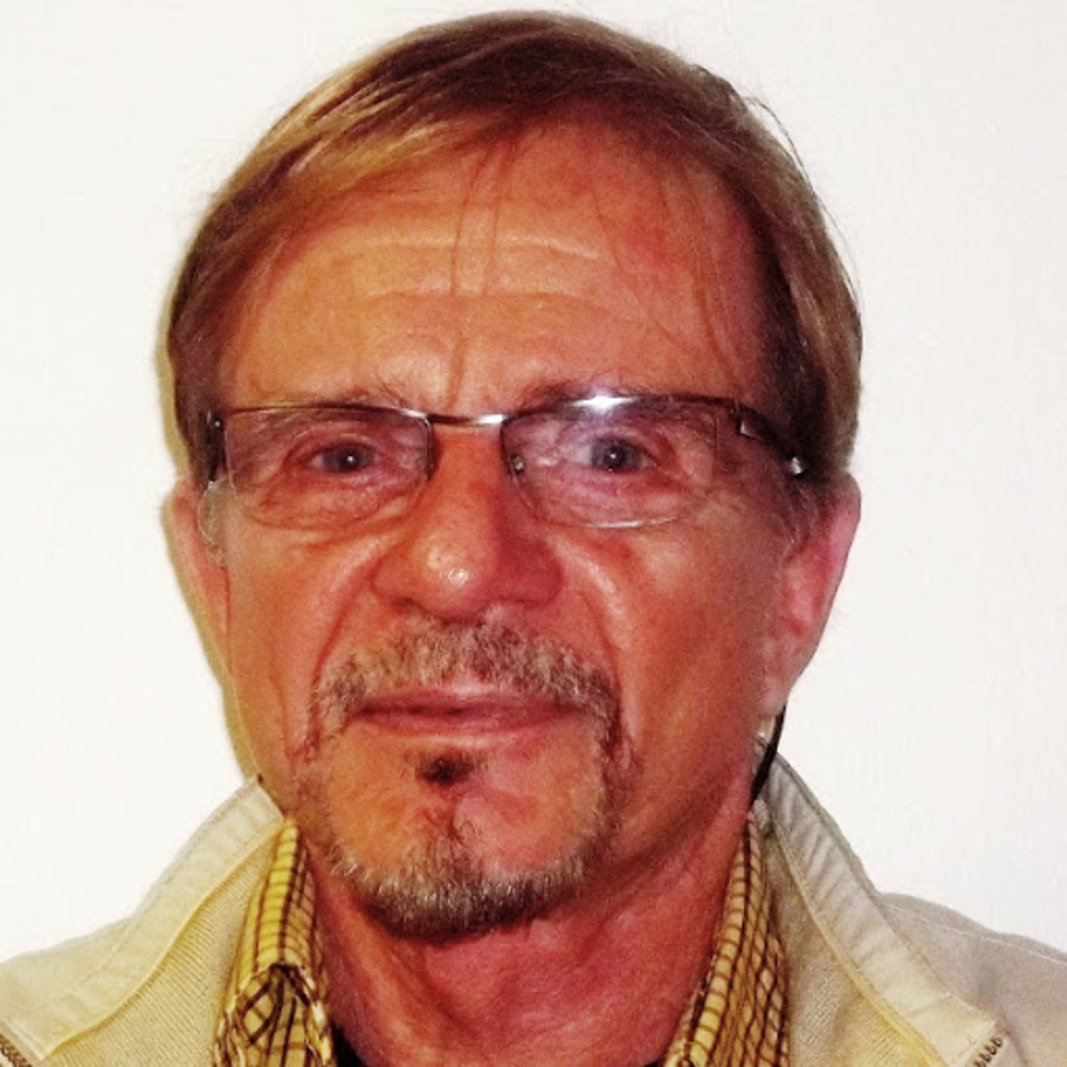
\includegraphics[width=0.15\textwidth]{figuras/igo.pdf}
\end{wrapfigure}

Caro Marcos Bacis Ceddia,

Gostei muito de seu artigo ``Mapeamento de Solos no nosso tempo'', publicado no número 2 do ``Pedometria Newsletter/SBCS'', no qual destaca a importância do uso de técnicas modernas nos levantamentos de solos.

No texto há a seguinte afirmação:

\begin{quotation}
  ``Sobre a ótica de modelos um mapa de solos pode ser entendido como um \textit{modelo da distribuição espacial de classes e/ou atributo de solos em uma determinada área de interesse}.''

\end{quotation}

É apenas um detalhe semântico, de menor importância, mas gostaria que ponderasse e nos respondesse, uma vez que tenho notado, em muitos trabalhos, alguma confusão entre Unidades de Mapeamento de Solo (que representam objetos reais) e Unidades Taxonômicas (representadas pelas classes):
Como em levantamentos pedológicos devemos considerar que o que mapeamos são objetos reais (os corpos de solos) e considerando que classes de solos são conceituais (isto é, abstrações, sem existência real) você considera correta a expressão ``distribuição espacial de classes de solos'' que usou em seu texto uma vez ser impossível ``mapear abstrações''?

Abraços.

\address{Igo F. Lepsch\\
  \begin{footnotesize}
    Pesq. Visistante; ICA-UFMG, Montes Claros, MG\\
    \email{igo.lepsch@yahoo.com.br}
  \end{footnotesize}
}
%%% Local Variables:
%%% mode: latex
%%% TeX-master: 3rd-edition.tex
%%% End:
\end{article}

\newpage

\begin{article}
   \title{Carta ao editor}
\subtitle{Réplica à Igo Lepsch sobre ``Mapeamento de Solos no nosso tempo''}
\author{por Marcos Ceddia}
\maketitle

\begin{wrapfigure}{l}{0.15\textwidth}
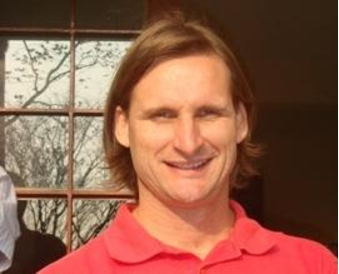
\includegraphics[width=0.15\textwidth]{figuras/marcos}
\end{wrapfigure}

Prezado Igo,

Obrigado pelas suas considerações. Embora o Sr. tenha comentado que sua pergunta talvez fosse ``um detalhe semântico, de menor importância'', dou, ao contrário, todo o valor à questão semântica. Se observarmos na literatura, muitas vezes detalhes semânticos geram confusões infindáveis que somente servem para criar mal entendidos de consequências inimagináveis. Por exemplo, por questões semânticas e interpretações das mais variadas, textos religiosos criaram barreiras intransponíveis entre seres humanos. Para Sócrates a ignorância é a origem do mal. De alguma forma, uma palavra mal colocada e mal interpretada contribui para a ignorância. No meio acadêmico também temos vários problemas, tais como: ensino equivocado, proliferação de versões não autorizadas, desvio da razão pelas quais se faz pesquisa, entre outras. Mais especificamente em Ciência do Solo, veja o problema que se criou quando o Mapeamento Digital de Solos iniciou!? Quanto problema gerou e ainda gera o termo ``Digital''? Por isso, não considero a discussão semântica uma perda de tempo ou de menor importância. Na verdade, sua pergunta abre uma grande oportunidade para rever conceitos, lembrar um pouco da história do levantamento e taxonomia de solos e, sobretudo, para desenvolver uma discussão contextualizada de questões tais como: Mapear classes ou atributos? Existe coerência entre a natureza do que mapeamos e a representação cartográfica dos mapas?

Assim, começamos pelos conceitos de Unidades de Mapeamento e Unidades Taxonômicas, afinal, os levantamentos pedológicos são executados com o apoio de sistemas taxonômicos de classificação.

\subsubsection{Unidade Taxonômica}

De acordo com os \textit{Procedimentos Normativos de Levantamentos Pedológicos} (EMBRAPA, 1995), uma Unidade Taxonômica é uma classe de solo definida e conceituada, segundo parâmetros de classificação. A conceituação é feita segundo um conjunto de características e propriedades do solo, conhecidas por meio de pedons e polipedons (uma entidade espacial). Uma unidade taxonômica corresponde à unidade de classificação mais homogênea em qualquer nível categórico de sistemas taxonômicos.

Aqui cabem algumas considerações. Como o senhor bem pontuou, uma Unidade Taxonômica é uma concepção teórica e é criada para facilitar o conhecimento sobre solos. Além disso, é uma concepção teórica passível de mudança, mais ou menos frequente, dependendo do sistema taxonômico que adotamos. O Sistema Brasileiro de Classificação de Solos (SiBCS), por exemplo, muda com muito mais frequência do que o sistema americano (Soil Taxonomy).

\subsubsection{Unidade de Mapeamento}

Unidades de mapeamento são áreas de solos definidas em função das unidades taxonômicas que as compõem. Trata-se de um conjunto de áreas de solos com relações e posições definidas na paisagem. Uma unidade de mapeamento é estabelecida e definida para possibilitar a representação cartográfica e mostrar a distribuição espacial de unidades taxonômicas.

Ao lermos o conceito de unidade de mapeamento (objetos reais que mapeamos e representamos no mapa), percebemos o quão estreita é a relação entre unidade taxonômica e unidade de mapeamento. Sem a unidade taxonômica, não existe a unidade de mapeamento com a nomenclatura que usamos, a qual é em essência uma concepção teórica. Uma perturbação relativamente frequente, a qual é consequência dessa estreita relação, é que comumente precisamos reclassificar os nomes que damos as unidades de mapeamento de cartas de solos.

Ainda, a relação entre unidade taxonômica e de mapeamento, recomento aos leitores o texto de Scull et al. (2003) intitulado \href{http://ppg.sagepub.com/cgi/content/abstract/27/2/171}{\textit{Predictive soil mapping: a review}}. Nesse trabalho, além de outros tópicos, o autor relembra a origem do sistema taxonômico de solos e o mecanismo utilizado para adequar a natureza altamente variante do solos e seus atributos com as limitações cartográficas da época. De acordo com Scull et al. (2003) o mapeamento de solos tem sido e continua sendo diretamente influenciado pelo processo de classificação do solo. O Autor cita o caso do Soil Taxonomy, o qual foi influenciado pela taxonomia biológica do século 19 e a prática do levantamento geológico. Aqui apresento a tradução exata do texto de Scull et al. (2003), onde fica bastante claro a estreita ligação entre unidades taxonômicas e unidades de mapeamento (trecho do segundo parágrafo da página 175).}

\begin{quotation}
  ``A proposta do Soil Taxonomy foi fornecer uma maneira objetiva para classificar sistematicamente o solo e foi adotado em uma época em que a informação do solo tinha que ser abstraída para o nível de perfil modal (classificado no Soil Taxonomy), porque era impossível catalogar e apresentar totalmente a variabilidade do solo. Com o objetivo de mapear as unidades taxonômicas, o solo tinha que ser distinguido como uma unidade espacial, um pedon (a menor unidade reconhecível que pode ser chamado de solo). Na prática, esta distinção espacial do solo resultou em um mapa onde as classes são unidades homogêneas com variabilidade desconhecida e limites pontuais (mapas coropléticos).''
\end{quotation}

Nesse ponto começamos a notar que também a Unidade de Mapeamento não pode ser considerada tão real assim, pois esta é na verdade uma maneira que os pedólogos criaram para representar espacialmente aquilo que se descreveu no campo e recebeu um nome teórico (nome da unidade taxonômica). Ou seja, sabe-se que o perfil modal não é homogêneo ao longo da paisagem (sua variação é contínua), mas o pedólogo (após explorar a área) elege alguns perfis modais para representar no mapa a distribuição espacial dos solos da área de estudo. A unidade de mapeamento passa a impressão de que consiste em um território homogêneo com limites abruptos. Sabemos que isso não é uma verdade, mas aceitamos como um ``modelo'' de representação espacial da distribuição dos solos (a carta de solos). Claramente, percebe-se que os mapas coropléticos não representam adequadamente a distribuição espacial da real variabilidade espacial dos solos. Importante notar que esse procedimento de mapeamento e representação cartográfica refletiu a disponibilidade tecnológica da época.

A partir do acima exposto também fica claro uma clara distinção entre o Mapeamento Digital de Solos e o Tradicional. Como a pesquisa em mapeamento digital de solo tem desenvolvido métodos de levantamento de solos que descrevem mais acuradamente a relação solo paisagem, comumente, tais métodos estão em desacordo com a abordagem tradicional. Os métodos digitais, frequentemente não adotam o conceito de solo como uma entidade espacial. Os métodos digitais estão mais focados no mapeamento da variabilidade espacial e temporal dos atributos dos solos (teor e estoque de carbono, retenção e disponibilidade de água, contaminantes e etc) e isso tem sido dificultado devido à defesa do Soil Taxonomy (Scull et al. 2003).

Após as considerações acima, agora retorno à sua pergunta referente ao termo que utilizei e que resultou em sua pergunta: ``Um modelo da distribuição espacial de classes e/ou atributo de solos em uma determinada área de interesse''. Na verdade o termo classes (o qual não fui eu o inventor) é utilizado para informar que o mapa (digital ou não) distingue espacialmente unidades de mapeamento que recebem o nome de uma unidade taxonômica. O modelo, nesse caso, representa a variabilidade espacial do solo com os ``defeitos'' da representação na forma de mapas coropléticos (percepção de variabilidade homogênea e com limites abruptos). Aqui podemos aproveitar para apresentar duas concepções de representação espacial que também geram polêmica, denominadas \textit{visão de objetos} e \textit{visão de campo}. Os mapas coropléticos seguem a visão de objetos, na qual as unidades de mapeamento (os objetos) são entidades independente no espaço. Na visão de campo (formato raster) a representação do mapa é feita através de uma matriz regular de linhas e colunas. Cada célula ou pixel recebe um valor (valor do atributo do solo ou classe de solo) e representa uma determinada área em função do tamanho de cada pixel (resolução). A visão de campo representa melhor o caráter contínuo da variabilidade espacial do solo. Além disso, é melhor para fazer análises espaciais em SIGs.

\subsubsection{Conclusões e considerações}

Podemos assim resumir que ao fazermos um mapa de classes de solos estamos representando o solo de forma irreal (a unidade de mapeamento não reflete a variabilidade espacial do solo) e também dando um nome que nada mais é que uma concepção teórica.

Minha humilde opinião é que os pesquisadores devem refletir melhor sobre a exata dimensão da taxonomia de solo sob o aspecto de mapeamento de solos. É inegável que com as tecnologias e ferramentas computacionais modernas obteve-se um ganho expressivo para se fazer levantamento e predição de atributos dos solos. Além disso, em muitos casos, o conhecimento da drenagem, disponibilidade de água, cor, teor de elementos químicos é de interpretação mais direta para um usuário do que dizer que uma parte do território á denominado por um nome taxonômico puramente teórico e voltado para fins acadêmico-científicos. Para um usuário de mapas de solos, uma mapa de classes de solos (tradicional ou digital) pode sim ser visto como um mapa abstrato.

\address{Marcos B. Ceddia\\
  \begin{footnotesize}
    Universidade Federal Rural do Rio de Janeiro\\
    \email{marcosceddia@gmail.com}
  \end{footnotesize}
}
%%% Local Variables:
%%% mode: latex
%%% TeX-master: 3rd-edition.tex
%%% End:
\end{article}

\newpage

\begin{article}
   \title{Carta ao editor}
\subtitle{Tréplica à Marcos Ceddia sobre ``Mapeamento de Solos no nosso tempo''}
\author{por Igo Lepsch}
\maketitle

\begin{wrapfigure}{l}{0.15\textwidth}
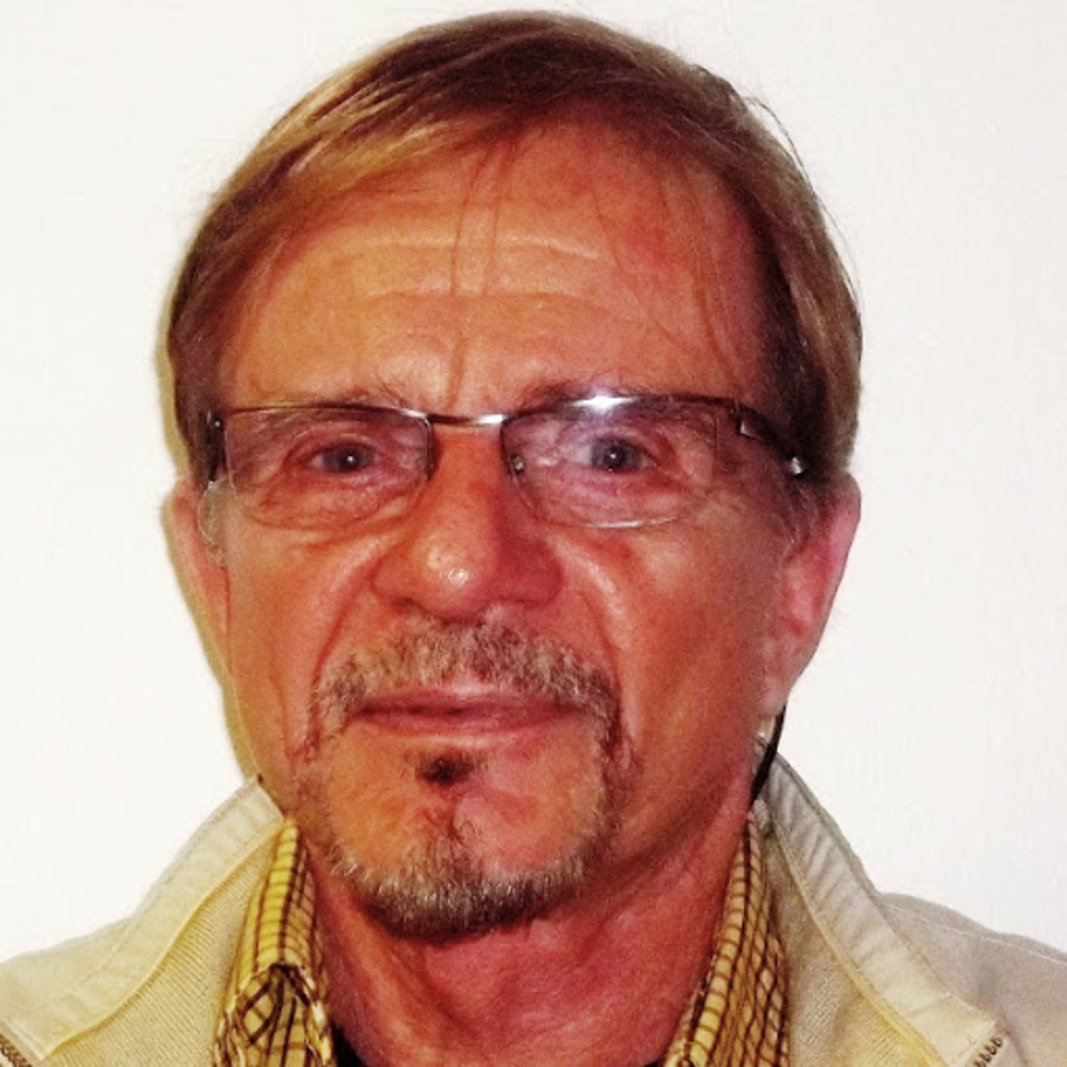
\includegraphics[width=0.15\textwidth]{figuras/igo}
\end{wrapfigure}

Caro Marcos,

Interessante as suas considerações. Quero completá-las com algumas citações e opiniões.

Nossa conversa começou com uma discussão sobre ``mapas de classes de solo'' e ``mapas de atributos do solo''. Você cita que Scull et al. (2003) é de opinião que o mapeamento de solos tem sido e continua sendo diretamente influenciado pelo processo de classificação do solo. Concordo com esses autores mas penso que um mapeamento de solos não deve ser influenciado por sistemas de classificação de solos.

Creio que os - por alguns autores - denominados ``mapas de classes de solos'' são na verdade mapas de indivíduos de solos ou simplesmente ``mapas de solos'' já que, em pedologia, solos são definidos como ``corpos naturais''.

Copiando algumas frases do livro de Jean-Paul Legros (\textit{Mapping of the Soil, 2006}):

\begin{quotation}
  ``Viewing soils as distinct individuals is very efficient from several points of view. To begin with, it allows us to structure our knowledge in the form of classifications. Then, it makes possible the drawing of maps on which boundaries appear. Thirdly, the entities thus shown can be processed by means of computer systems suitable for the creation of categorical maps. But some authors judge this attitude rather harshly: \textit{`The survey and classification of geology, soil or vegetation into exact, sharply defined} classes \textit{or areas that meet abstract ideas of nicely defined, properly circumscribed} units \textit{has been an enormous exercise in forcing continuously varying phenomena into exact moulds. Although much scientific evidence has been assembled to demonstrate that} soils \textit{are not exact, homogeneous entities[...]'''}(Burrough and Franck, 1995).
\end{quotation}

Legros (2006) afirma que nem todos autores concordam com o corpo de solo tal como maioria dos pedólogos o define. Contudo, a maior parte dos pedólogos, que durante muitos anos mapearam - em detalhe - solos no campo usando conhecimentos tácitos, acreditam realmente que ''indivíduos solo'' existam; e eles os tem delineado em muitos mapas de muitas regiões. Em respeito a esses colegas consideremos que os corpos de solo existam mesmo e que os delineamentos que fazemos nos mapas e que mais se aproximam destes corpo natural sejam as séries de solo.

Temos que considerar também que um trabalho, que visa à compreensão e modelagem da natureza, só será social e economicamente justificado se os relatórios correspondentes puderem ser aplicados (ou seja, se incluírem interpretações para usos práticos).

Consideremos agora que, para que um mapa de solos tenha aplicação prática ele deve ser feito numa escala que possa ser útil aos usuários; isto é, deve ser um levantamento detalhado, definido como aquele que deve ser executado ``em nível de séries''. Há que ponderar também que os relatórios desses levantamentos, para terem seu custo justificado, devem incluir interpretações para agricultura, engenharia civil, etc (tal como os relatórios dos ``soil surveys'' dos EUA).

No Brasil - ao contrário de muitos outros países (como EUA e os nosso vizinhos argentinos) - série de solos ainda não foram definidas, raros são os levantamentos detalhados executados por órgãos do Governo e raros também são os relatórios que apresentam aplicações para usos práticos.

O país que mais executou levantamentos detalhados e mais os usa para fins práticos é os EUA. Em 1960 boa parte do território americano já estava mapeada (escalas próximas de 1:30.000) com mais de dez mil séries identificadas. E esses mapas não eram de classes de solos, uma vez que séries de solos só foram consideradas como classes após o aparecimento do ``Soil Taxonomy''. Mesmo assim, houve muitas dúvidas se séries de solos deviam ser consideradas como classes ou não. Abaixo algumas frases copiadas de uma \href{http://www.nrcs.usda.gov/wps/portal/nrcs/detail/soils/planners/?cid=nrcs142p2_053571}{nota técnica do USDA-NRCS} que informa sobre isso.

\begin{quotation}
  ``Today we readily accept that a soil series is the lowest level of Soil Taxonomy and its properties can not extend beyond the limits of the family to which it belongs. This was not always so easily accepted. The 1965 NCSS conference proceedings includes a discussion of \textit{guidelines for allowable tolerances in the stretching of family class limits by series class limits}. The debate was whether the range in characteristics for a series must be within the limits of the family, or alternatively, should only the typical pedon itself have to fit within the family while its range could extend beyond the family limits. The first alternative was agreed to.
    
  The decision to restrict series ranges to family limits has presented some difficulty ever since. We know that natural soil bodies commonly have ranges in properties that straddle one or more of the rigid taxonomic class boundaries. Over the years we have used devices such as taxadjuncts, variants, and \textit{similar soils} to reconcile observations from natural bodies of soils with taxonomic limits. These concepts are awkward and not well understood beyond the soil survey community. In 1977 Dr. Marlin Cline wrote \textit{At the lowest level of the system, we will have to acknowledge the differences between taxonomic soil series and mapping units that bear the same name and will probably have to rectify the confusion this causes. It is conceivable that soil families could become the lowest category of taxonomy, but some ingenious person may find a better solution.}''
\end{quotation}

E, mais adiante:

\begin{quotation}
  ``The distinction between taxonomic classes and components of map units needs to be understood. \textbf{We do not map taxonomic classes} [grifo meu]. We use conceptual landscape models to map natural bodies of soils. We then use our taxonomy to classify and name the soils we have mapped.''   
\end{quotation}

Portanto, creio que: se o mapeamento de solos tem sido e continua sendo diretamente influenciado pelo processo de classificação do solo e se o ``Soil Taxonomy'' é a classificação mais usada, creio que é porque está havendo confusão entre Unidade de Mapeamento (que são objetos) e Unidade Taxonômica (que são conceitos abstratos). Vale a pena ler algo sobre isso no \href{http://casoilresource.lawr.ucdavis.edu/w/images/d/d8/CHAPTER_5_Application_of_Soil_Taxonomy_to_Soil_Surveys.pdf}{capítulo 5} da Nova Edição do ``Soil Taxonomy'':

\begin{quotation}
  ``Soils are landscapes as well as profiles (USDA, SCS, 1951, pp. 5-8; USDA, SCS, 1993, pp. 9-11). In soil survey, a soil-landscape unit can be thought of as a landscape unit (landscape, landform, or landform component) further modified by one or more of the soil-forming factors. Within a soil-landscape unit, the five factors of soil formation interact in a distinctive manner. As a result, areas of a soil-landscape unit have a relatively homogeneous soil pattern. A soil surveyor perceives soil patterns by first conceptually dividing the landscape into soil-landscape units. The boundaries between dissimilar soil-landscape units are placed where one or more of the soil-forming factors change within a short lateral distance.''
\end{quotation}

Convém informar que o Comitê executivo do Sistema Brasileiro de Classificação de Solos (SiBCS) está revendo a conceituação de séries como Unidade Taxonômica. Muitos países que já tem suas séries de solo definidas mas, não as consideram como classes. Provavelmente as primeiras séries de solo brasileiras não serão classes (ou táxons) tal como não o foram as milhares primeiras séries dos EUA. Afinal, para que uma série se solo seja ``batizada'' é necessário que primeiro ela tenha uma área mínima mapeada (normalmente 1.000 ha). Se assim for, e considerando como correta a expressão da nota técnica número quatro do USDA-NRCS de que ``[...] we do not map taxonomic classes[...], we use conceptual landscape models to map natural bodies of soils[...]'', como primeiro conceituar ``séries classes'' sem antes termos ``séries unidade de mapeamento''? Como definir conceitos sem termos os objetos?

Com respeito a suas observações sobre caracterização das unidades de mapeamento, que hoje muitos fazem o que chamam ``perfil representativo'', isso é uma preocupação de longa data. Sobre isso veja alguns comentários de S. W. Buol em \href{http://base.dnsgb.com.ua/files/book/Agriculture/Soil/Soil-Classification.pdf}{``Philosophies of Soil Classifications: From is to does''}:

\begin{quotation}
  ``Cursorily observation of a soil reveals a vertical arrangement of soil components that change, often gradually, as one traverses the landscape. Our understanding of soil is limited without utilization of chemical, mineralogical, biological and physical quantification of soil samples. Soil can be dismembered, sampled and autopsied but only if we know from where each soil sample is located within a body of soil do the analyses help us understand both what a soil is and what a soil does. Identification of depth and vertical arrangement of a soils component parts via several degrees of sophistication i.e. topsoil, subsoil, generic horizon nomenclature and diagnostic horizons is endemic to all attempts to classify soil.

  Perhaps no single problem has plagued soil classification more than identification of the spatial boundaries of a soil individual on the landscape that is to be sampled for study and used as a unit of classification. As soil science struggled to claim adulthood as an independent science a basis of identifying a soil individual suitable for classification has been at the root of many philosophies. Soil classification is closely allied with soil mapping and most practitioners intertwined pragmatic realities of mapping into their philosophies of identifying an appropriate volume of soil for classification''.
\end{quotation}

Creio que a pedometria pode nos ajudar muito a identificar o melhor local para amostrar os ``perfis modais'' depois que as unidades de mapeamento de solos forem delineadas com base em modelos conceituais solo-paisagem. Perfis estes que realmente represente nosso objeto de estudo: os corpos naturais dos solos. Por vezes, tenho a impressão que muito do que chamamos ``perfis representativos'' são escolhidos mais para representar conceitos (classes definidas no SiBCS) do que os objetos que mapeamos. Sobre essa problemática veja o que afirmamos \href{http://www.e-publicacoes.uerj.br/index.php/tamoios/article/view/5665/5196}{em um artigo nosso}:

\begin{quotation}
  ``Com a ênfase em características dos perfis do solo muitos pedólogos brasileiros tendem a ter uma ``visão afunilada'' das terras considerando muito mais os perfis expostos em trincheiras abertas em um único local do corpo do solo sem tentar integrá-lo na paisagem como um todo. Em outras palavras a atenção maior tem sido na IMAGEM (perfil do solo) e CONCEITO (classificação) deixando o OBJETO (corpo de solo) em segundo plano.''
\end{quotation}

\address{Igo F. Lepsch\\
  \begin{footnotesize}
    Pesq. Visistante; ICA-UFMG, Montes Claros, MG\\
    \email{igo.lepsch@yahoo.com.br}
  \end{footnotesize}
}
%%% Local Variables:
%%% mode: latex
%%% TeX-master: 3rd-edition.tex
%%% End:

\end{article}

\newpage

\begin{article}
   \title{Um pouco de R na \textit{Newsletter}}
\subtitle{Nuvem de palavras}
\author{por Alessandro Samuel-Rosa}
\maketitle
\begin{wrapfigure}{l}{0.15\textwidth}
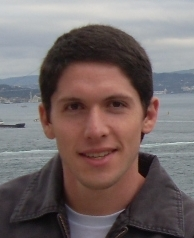
\includegraphics[width=0.15\textwidth]{figuras/foto-alessandro}
\end{wrapfigure}
O ambiente de análise de dados \R{} possui uma imensidade de funcionalidades que vão desde simples operações algébricas até a modelagem de complexas relações entre o solo e os fatores de formação do solo. Um bom exemplo do último caso é mostrado acima no artigo do Waldir, do Cesar e da Michele sobre a disciplina de mapeamento digital de solos ministrada na Universidade Federal Rural do Rio de Janeiro. Mas o que poucos sabem é que, sendo um ambiente de análise de dados, e não um simples software estatístico, quaisquer tipos de dados podem ser analisados no \R{}. Isso inclui dados contínuos, categóricos, imagens, vetores, volumes, 1D, 2D, 3D, 4D, áudio, vídeo, texto, e mais uma infinidade de possibilidades. Mas hoje vou me deter à apenas um destes tipos de dados, os dados textuais.
\subsection{Nuvem de palavras}
No presente número da \textit{Newsletter} da Comissão de Pedometria, uma novidade foi apresentada na página de abertura: um logo formado por uma nuvem de palavras.\\
\\
\emph{Uma nuvem de palavras, ou nuvem de tags, é uma representação visual de dados textuais onde a importância de cada palavra no texto é mostrada com o tamanho da fonte ou cor} \citep{wiki:2013}.\\
\\
Os dados textuais utilizados aqui são representados pelo conteúdo do seguinte vetor:
\begin{smallverbatim}
 > words <- c("pedometria pedometria pedometria
 pedometria solo estatística matemática sensores
 pedologia mapeamento gênese espaço variabilidade
 amostra dados métodos variação informática
 tecnologia programação script amostragem GPS
 satélite MDE pedólogo regressão geoestatística
 pedotransferência modelos resíduo incerteza
 computador mapas covariáveis tempo 3D função
 validação calibração SIG sistema predição
 interpolação ajuste curva rede neural árvore
 decisão classificação especialista erro
 correlação seleção automático paisagem logística
 simulação terreno atributo geologia clima imagem
 pixel escala resolução ensino pesquisa extensão
 agricultura ambiente precisão acurácia")
\end{smallverbatim}
A composição do vetor de dados textuais foi definida a partir da minha memória dos termos mais relacionados à pedometria. Como minha memória é falha e enviesada pelas minhas experiências pessoais, é provável que muitos outros termos poderiam ter sido incluídos. Sugestões são bem vindas para preparar o logo dos próximos números da \textit{Newsletter}. Além disso, outros dados textuais também podem ser analisados, como por exemplo o conteúdo textual de um artigo, livro ou até mesmo da \textit{Newsletter}. Como fazer isto é o que eu mostro abaixo.
\subsection{Instalando os pacotes necessários}
\label{subsec:pacotes}
Os pacotes necessários para a elaboração de uma nuvem de palavras, como aquela usada como logo da \textit{Newsletter}, são quatro: \texttt{wordcloud} \citep{Fellows:2013}, \texttt{tm} \citep{FeinererEtAl:2013}, \texttt{slam} \citep{HornikEtAl:2013}, e \texttt{RColorBrewer} \citep{Neuwirth:2011}. O pacote \texttt{wordcloud} é aquele que gera a nuvem de palavras usado como logo da \textit{Newsletter}. Já os pacotes \texttt{tm} e \texttt{slam} são dependências do pacote \texttt{wordcloud} usados na análise dos dados para a geração da nuvem de palavras. Para instalar e carregar estes pacotes basta usar os comandos:
\begin{smallverbatim}
> install.packages(c("wordcloud","tm", "slam",
"RColorBrewer"),
> repos = "http://cran.r-project.org")
> require(wordcloud)
> require(RColorBrewer)
\end{smallverbatim}
\subsection{Definindo a paleta de cores}
Depois de instalados e carregados os pacotes, define-se a paleta de cores usando o pacote \texttt{RColorBrewer}. São diversas as opções de paletas de cores do pacote \texttt{RColorBrewer}, cuja demonstração está além do objetivo deste artigo. Maiores informações podem ser encontradas acessando o endereço \url{http://colorbrewer2.org/}. No caso da nuvem de palavras usada como logo da \textit{Newsletter}, a paleta usada foi aquela identificada como \texttt{YlOrBr}, que varia entre as cores amarelo (\emph{yellow}), laranja (\emph{orange}) e marrom (\emph{brown}). O comando usado é o seguinte:
\begin{smallverbatim}
> pal <- brewer.pal(n = 9, name = "YlOrBr")
\end{smallverbatim}
\subsection{Gerando a nuvem de palavras}
Carregados os pacotes necessários, definidos os dados textuais e a paleta de cores, agora é possível invocar a função \texttt{wordcloud} para gerar a nuvem de palavras:
\begin{smallverbatim}
> wordcloud(words = words, min.freq = Inf,
random.order = FALSE, random.color = TRUE,
colors = pal, rot.per = 0.2, fixed.asp = TRUE)
\end{smallverbatim}
Os parâmetros fornecidos ao comando \texttt{wordcloud} definem o objeto do \R{} contendo os dados textuais (\texttt{words = words}), não havendo limite de frequência mínima para que um termo que aparece nos dados textuais seja apresentado graficamente (\texttt{min.freq = Inf}). Os termos são apresentados no gráfico em ordem decrescente de frequência (\texttt{random.order = FALSE}) e as cores da paleta (colors = pal) são atribuídas aleatoriamente (\texttt{random.color = TRUE}). Apenas 20\% dos termos podem ser apresentados graficamente na vertical (\texttt{rot.per = 0.2}), dando-se preferência pela apresentação gráfica com a relação de aspecto dos eixos x e y fixa (\texttt{fixed.asp = TRUE}).
\subsection{Salvando a nuvem de palavras como figura}
Depois de gerada a nuvem de palavras, existem diversas maneiras de salvar uma figura para usar, por exemplo, no cabeçalho da \textit{Newsletter}. A primeira opção é salvar um arquivo no formato *.pdf usando o seguinte comando:
\begin{smallverbatim}
> pdf(file = "wordcloud.pdf")
> wordcloud(words = words, min.freq = Inf,
random.order = FALSE, random.color = TRUE,
colors = pal, rot.per = 0.2, fixed.asp = TRUE)
> dev.off()
\end{smallverbatim}
A segunda opção é salvar um arquivo no formato *.png usando o seguinte comando:
\begin{smallverbatim}
> x11(width = 17/2.5, height = 7.5/2.5,
bg = "black")
> wordcloud(words = words, min.freq = Inf,
random.order = FALSE, random.color = TRUE,
colors = pal, rot.per = 0, fixed.asp = FALSE)
> savePlot(filename = "wordcloud-black.png")
> dev.off()
\end{smallverbatim}
Note que o arquivo salvo no formato *.png possui algumas peculiaridades, como por exemplo o uso do comando \texttt{x11()} para definir uma região de apresentação gráfica com $17/2.5$ polegadas de largura e $7.5/2.5$ polegadas de altura, com plano de fundo preto (\texttt{bg = "black"}). Além disso, nenhum termo foi permitido aparecer na vertical e a relação de aspecto dos eixos x e y foi mantida livre (\texttt{rot.per = 0} e \texttt{fixed.asp = FALSE}). Os produtos gráficos são mostrados pelas figuras \ref{fig:wordcloud} e \ref{fig:wordcloud-black}.\\
\\
\begin{figure}[htbp]
   \centering
   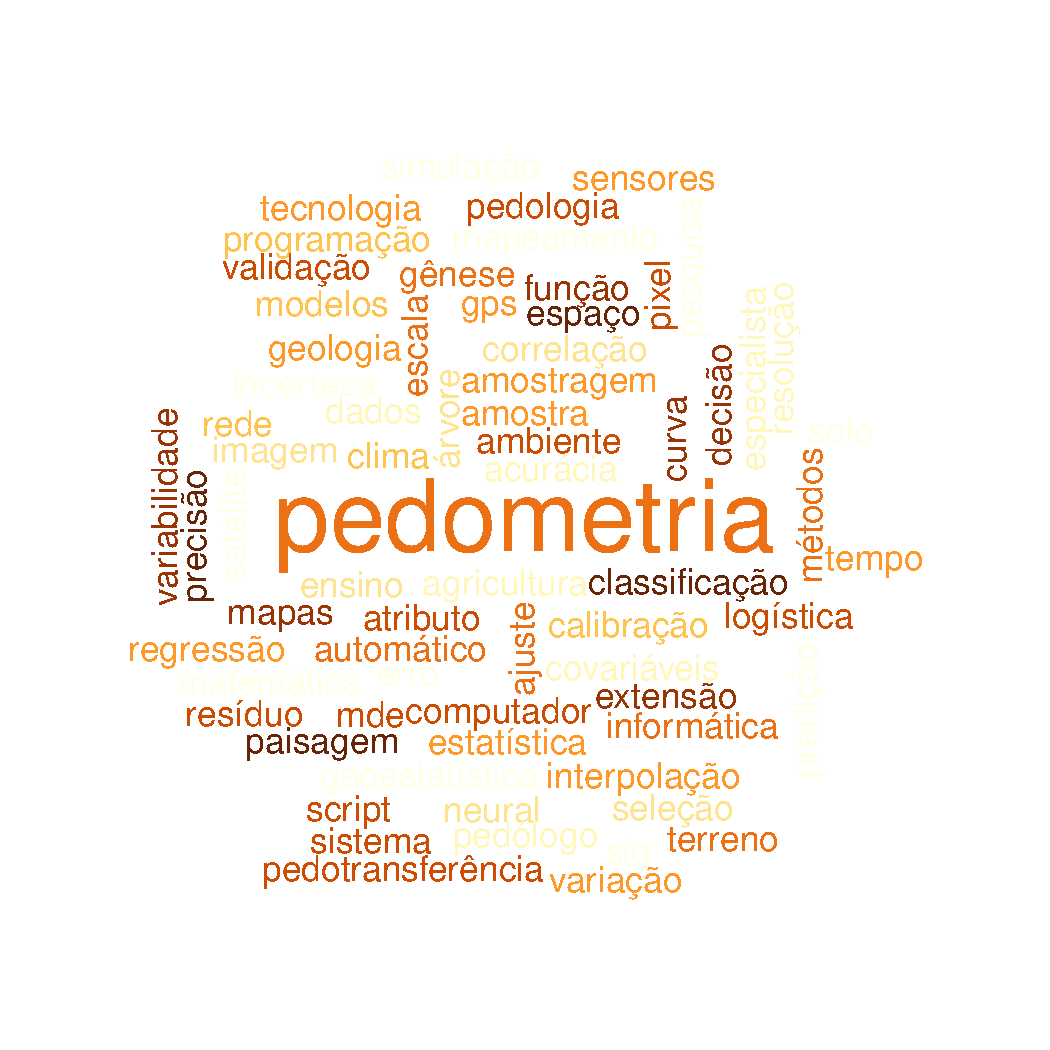
\includegraphics[scale=0.8]{figuras/wordcloud}
   \caption{Nuvem de palavras ligadas à pedometria com fundo branco e relação de aspecto fixa.}
   \label{fig:wordcloud}
\end{figure}
\noindent Diversas alterações podem ser feitas no produto gráfico final simplesmente alterando o conteúdo do vetor de dados textuais. Para aumentar ainda mais o tamanho do termo ``pedometria'' em relação aos demais termos, basta repeti-lo mais algumas vezes. Da mesma forma, se quisermos dar ênfase a outros termos, como por exemplo ``matemática'' e ``estatística'', basta repeti-los mais algumas vezes.\\
\\
\begin{figure}[htbp]
   \centering
   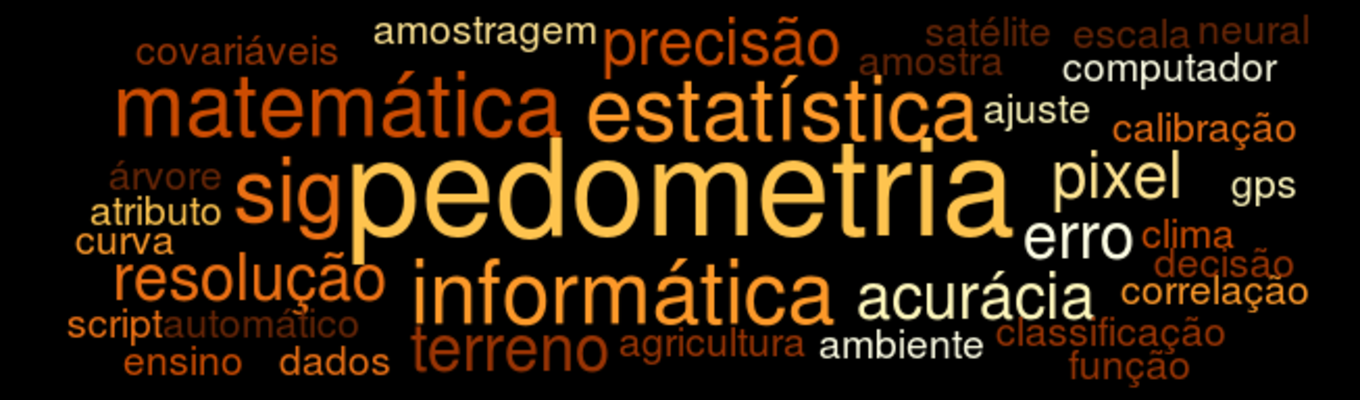
\includegraphics[scale=0.8]{figuras/wordcloud-black}
   \caption{Nuvem de palavras ligadas à pedometria com fundo preto e relação de aspecto livre.}
   \label{fig:wordcloud-black}
\end{figure}
\subsection{Um pouco de \R{} na \textit{Newsletter}}
Como eu disse no início deste artigo, existem diversos termos que poderiam ter sido acrescentados ao meu objeto contendo os dados textuais. Tais termos não foram incluídos simplesmente porque eu não lembrei deles ou porque não fazem parte do conjunto de termos que costumo relacionar à pedometria. É por este motivo que aqueles que gostarem de ver outros termos na nuvem de palavras que compõe o logo da \textit{Newsletter}, por favor, não exitem em entrar em contato pelo endereço de e-mail \email{alessandrosamuel@yahoo.com.br}. Ao mais aventureiros, o script usado no \R{} para produzir a nuvem de palavras pode ser baixado \href{http://goo.gl/tqGmI1}{clicando aqui} e usado para gerar novas e diferentes nuvens de palavras.
\begin{footnotesize}
\begin{thebibliography}{99}
\bibitem[Wikipedia (2013) Wikipedia]{wiki:2013}
Wikipedia (2013)
\newblock Tag cloud --- Wikipedia, The Free Encyclopedia.
\newblock \url{http://en.wikipedia.org/w/index.php?title=Tag_cloud&oldid=571203887} [Online; accessed 8-October-2013].
\bibitem[Fellows (2013) Fellows]{Fellows:2013}
I. Fellows (2013)
\newblock wordcloud: Word Clouds.
\newblock \url{http://CRAN.R-project.org/package=wordcloud} [R package version 2.4]
\bibitem[Feinerer \& Hornik (2013) Feinerer \& Hornik]{FeinererEtAl:2013}
I. Feinerer \& K. Hornik (2013)
\newblock tm: Text Mining Package.
\newblock \url{http://CRAN.R-project.org/package=tm} [R package version 0.5-9.1]
\bibitem[Hornik et~al. (2013) Hornik, Meyer \& Buchta]{HornikEtAl:2013}
K. Hornik, D. Meyer \& C. Buchta (2013)
\newblock slam: Sparse Lightweight Arrays and Matrices.
\newblock \url{http://CRAN.R-project.org/package=slam} [R package version 0.1-30]
\bibitem[Neuwirth (2011) Neuwirth]{Neuwirth:2011}
E. Neuwirth (2011)
\newblock RColorBrewer: ColorBrewer palettes.
\newblock \url{http://CRAN.R-project.org/package=RColorBrewer} [R package version 1.0-5]
\end{thebibliography}
\end{footnotesize}
\address{Alessandro Samuel-Rosa\\
  Universidade Federal Rural do Rio de Janeiro\\
  \url{soil-scientist.net}\\
  \email{alessandrosamuel@yahoo.com.br}}
%%% Local Variables: 
%%% mode: latex
%%% TeX-master: documento-principal.tex
%%% End: 
\end{article}

\newpage

\begin{article}
   \title{Eventos}
\maketitle


\section{INTERGEO}
\subsection{Istambul, Turquia, 28-29/4/2014}
O congresso é organizado pela German Society of Geodesy, Geoinformation and Land Management (DVW). 
Maiores informações podem ser encontradas no endereço \url{http://www.intergeo-eurasia.net/en/index.html}.


\section{Conferência e Feira de Geomática e Soluções Geoespaciais}
\subsection{São Paulo, Brasil, 7-9/5/2014}
O evento é organizado por MundoGEO.
Maiores informações podem ser encontradas no endereço \url{http://mundogeoconnect.com/2014/}.


\section{ISRIC'S Spring School 2014}
\subsection{Wageningen, Holanda, 12-16/5/2014}
O evento é organizado pelo International Soil Reference and Information Centre - ISRIC. Serão abordados temas relacionados ao Mapeamento Digital de Solos (MDS) e uso de softwares para análise de dados de solos.
Maiores informações podem ser encontradas no endereço \url{http://www.isric.org/content/isrics-spring-school-2014}.


\section{20th Word Congress of Soil Science}
\subsection{Jeju, Korea, 8-13/06/2014}
O congresso é organizado pela International Union of Soil Sciences (IUSS). 
Maiores informações podem ser encontradas no endereço \url{http://www.20wcss.org/}.


\section{12th International Conference of Precision Agriculture}
\subsection{Sacramento, Califórnia (USA), 20-23/07/2014}
O congresso é organizado pela Sociedade Internacional de Agricultura de Precisão.
Maiores informações podem ser encontradas no endereço \url{https://www.ispag.org/ICPA/}.


\section{XX Congresso Latinoamericano de la Ciencia Del Suelo}
\subsection{Cusco, Perú, 9-15/11/2014}
O evento é organizado pela Sociedade Latinoamericana de Ciência do Solo (SLCS).
Maiores informações podem ser encontradas no endereço \url{http://www.xxcongresolatinoamericanodesuelosperu.org/programa.php}.


\section{6th Global Workshop on Digital Soil Mapping}
\subsection{Nanjing, China, 11-14/11/2014}
O evento é  organizado pelo Instituto de Ciência do Solo da Academia Chinesa de Ciências. O prazo para submissão de trabalhos é 31/07/2014.
Maiores inforamçoes podem ser encontradas no endereço \url{http://dsm2014.csp.escience.cn/}.


\address{Jean Michel Moura-Bueno\\
    Universidade Federal de Santa Maria\\
    \email{bueno.jean1@gmail.com}}
\end{article}

\begin{article}
   \title{Instruções aos autores}
\maketitle
\newcommand{\SBCS}{\href{http://www.sbcs.org.br/}{SBCS}}
\newcommand{\Nature}{\href{http://www.nature.com/nature/authors/gta/}{Nature}}
\newcommand{\Science}{\href{http://www.sciencemag.org/about/authors}{Science}}
\newcommand{\CreativeCommons}{\href{http://creativecommons.org/licenses/by-sa/2.0/}{CC-BY-SA}}
\newcommand{\Kile}{\href{http://kile.sourceforge.net/}{Kile}}
\newcommand{\MiKTeX}{\href{http://miktex.org/}{MiKTeX}}
\newcommand{\aquiLaTeX}{\href{https://docs.google.com/document/d/1F3IXzWNCeUrwKeFxA4iHS3aw1nforK1IqB126xbawvA/edit?usp=sharing}{aqui}}
\newcommand{\aquiWord}{\href{https://docs.google.com/document/d/1pyK03RBDPhOMrTVfvj9NcEfjGWeswqYbYDqEKq83drQ/edit?usp=sharing}{aqui}}
\newcommand{\Geoderma}{\href{http://www.elsevier.com/author-schemas/latex-instructions}{Geoderma}}
\newcommand{\EJSS}{\href{http://onlinelibrary.wiley.com/journal/10.1111/\%28ISSN\%291365-2389/homepage/ForAuthors.html}{European Journal of Soil Science}}

\subsection{Escopo e política}

\pedometria{} é a \textit{Newsletter} (boletim técnico-científico) da Comissão de Pedometria da Sociedade Brasileira de Ciência do Solo (\SBCS). Assim sendo, dedica-se à publicação de artigos relacionados à aplicação de métodos matemáticos e estatísticos para o estudo da gênese e distribuição dos solos, o que abrange desde discussões conceituais até a aplicação prática de sensores e modelos. Especificamente, os seguintes tópicos costumam ser cobertos:

\begin{itemize}
 \item explicitação de conceitos pedométricos;
 \item entrevista com pedometrista;
 \item opinião sobre tema pedométrico relevante;
 \item descrição de equipamentos e sensores remotos;
 \item descrição de softwares e suas funcionalidades;
 \item eventos técnico-científicos;
 \item expressão artística em pedometria;
 \item novas publicações científicas em pedometria.
\end{itemize}

Os artigos submetidos para publicação em \pedometria{} NÃO DEVEM ser formais como aqueles geralmente submetidos para revistas científicas tradicionais da área de pedometria. DEVE-SE usar linguagem CLARA e INFORMAL, preferencialmente na VOZ ATIVA. O uso da voz ativa é uma recomendação para publicação em ambas as revistas \Nature{} e \Science:

\begin{description}
 \item \textit{Nature} ``Nature journals like authors to write in the active voice (`we performed the experiment...') as experience has shown that readers find concepts and results to be conveyed more clearly if written directly.''
 \item \textit{Science} ``Use active voice when suitable, particularly when necessary for correct syntax (e.g., `To address this possibility, we constructed a lZap library ...,' not `To address this possibility, a lZap library was constructed...').''
\end{description}

Conceitos pedométricos devem ser introduzidos com SENSIBILIDADE, tendo em mente que os leitores podem os desconhecer e/ou não possuir base conceitual suficiente para compreendê-los em uma única leitura. A estrutura do artigo deve ser concebida da mesma maneira que o fazemos para contar uma história a um amigo ou familiar, a fim de cativar o leitor e envolvê-lo no emocionante universo da pedometria. Caso a comissão editorial entenda que a compreensão do texto exija aprofundado conhecimento prévio do leitor, os autores serão solicitados a torná-lo mais simples e amigável.

O escopo e política de \pedometria{} coloca-a como veículo de divulgação e desmistificação da pedometria no Brasil. Trata-se de uma publicação com três edições anuais que permite aos pesquisadores brasileiros divulgar suas pesquisas pedométricas e, sobretudo, conhecerem uns aos outros. Isso é importante porque, assim como a própria pedometria, a maioria dos pedometristas também são bastante jovens, muitos dos quais ainda estão desenvolvendo seus estudos de mestrado e/ou doutorado. Por este motivo, \pedometria{} é distribuída gratuitamente via Internet, estando registrada sob a licença Creative Commons Atribuição-Compartilha Igual 3.0 Não Adaptada (\CreativeCommons).\\
\\
\begin{figure}[h!]
 \centering
 
\includegraphics[width=0.8\textwidth]{figuras/cc-by-sa}
 \caption{Licença Creative Commons Atribuição-Compartilha Igual 3.0 Não Adaptada.}
\end{figure}

\subsection{Estrutura do artigo}

A estrutura do artigo é inteiramente definida pelo(s) autor(es). Sugere-se que sejam utilizadas subdivisões em até dois níveis de profundidade (seções e subseções), não necessariamente definidas como em artigos científicos tradicionais. Os artigos podem ter, além do título, um subtítulo. Resumo e palavras-chave não são utilizados.

\subsubsection{Figuras e tabelas}

Figuras e tabelas são recomendadas, sendo uma foto do(s) autor(es) obrigatória. Figuras devem ser preparadas no formato PNG, com resolução mínima de 300 dpi.

\subsubsection{Referências bibliográficas}

Referências bibliográficas não são mandatórias, sobretudo no caso de artigos apresentando a opinião do autor sobre um tema pedométrico. Caso citações sejam feitas ao longo do texto, a lista de referências deve ser organizada na ordem em que as citações são feitas no texto. Importante notar que o estilo de citação numérica sobrescrita da \textit{Nature} é utilizado.

A lista de referências bibliográficas deve conter até cinquenta itens. O conteúdo da lista de referências deve ser econômico, incluindo apenas informações fundamentais para a sua identificação. Artigos, trabalhos em anais de eventos ou em coleções, e trabalhos publicados em veículos periódicos similares, devem ser formatados da seguinte maneira:

\vspace{0.5cm}
\noindent{A.B. McBratney, M.L. Mendonça-Santos, B. Minasny (2003) On digital soil mapping. \textit{Geoderma}, 117:3-52. \doi{10.1016/S0016-7061(03)00223-4}}
\vspace{0.5cm}

\noindent{onde \textit{link} refere-se ao endereço na Internet onde o referido documento pode ser encontrado. No caso de artigos científicos recomenda-se utilizar o Digital Object Identifier (\href{http://www.doi.org/}{DOI}). Livros, teses, dissertações, relatórios e outros meios de publicação não periódicos devem ser formatados da seguinte maneira:}

\vspace{0.5cm}
\noindent{H. Jenny (1994) \textit{Factors of soil formation - a system of quantitative pedology}. Toronto: Dover Publications.}
\vspace{0.5cm}

\noindent{Caso as publicações não periódicas estejam disponíveis na Internet, um link deve ser adicionado assim como para as publicações periódicas.}

\subsection{Preparo do artigo}

Os artigos podem ser preparados utilizando processadores de texto tradicionais, como por exemplo o MS Office Word (*.doc) e o LibreOffice Writer (*.odt), ou a linguagem de marcação \LaTeX() (*.tex). Preferência deve ser dada ao formato \LaTeX() sempre que possível a fim de facilitar o trabalho da equipe editorial. Documentos no formato PDF não são aceitos.

\subsubsection{Word ou Writer}

Um modelo para preparo do artigo usando processadores de texto tradicionais pode ser acessado clicando \aquiWord.

\subsubsection{\LaTeX}

\href{http://pt.wikipedia.org/wiki/Latex}{\LaTeX} é uma \href{http://pt.wikipedia.org/wiki/Linguagem_de_marca\%C3\%A7\%C3\%A3o}{linguagem de marcação} amplamente utilizada para a produção de textos matemáticos e científicos devido à sua alta qualidade tipográfica. Utilizar uma linguagem de marcação para elaboração de textos constitui no uso de comandos escritos para definir a formatação do documento, ao contrário dos editores tradicionais que oferecem abas e caixas de diálogo para clicar e definir parâmetros de formatação. Na prática, ao produzir um texto em \LaTeX, o autor não vê o produto final formatado na tela do computador imediatamente, mas apenas o texto e os comandos de formatação. O objetivo é distanciar o autor o máximo possível da apresentação visual do artigo, ou seja, ao invés de trabalhar com ideias visuais, o autor é encorajado a trabalhar com conceitos lógicos independentes da apresentação final do artigo. Além disso, linguagens de marcação como o \LaTeX{} permitem agilizar a confecção do documento final (PDF) e reproduzir o conteúdo em outros formatos para apresentação em meio digital como o html. Atualmente, importantes revistas científicas da área de pedometria adotam o \LaTeX{} para a confecção de seus artigos, como por exemplo \Geoderma{} e \EJSS.

Apesar de diferente dos processadores de texto tradicionais, usar \LaTeX{} é bastante fácil, sendo necessário apenas compreender a sua lógica de funcionamento. Para isso é bom dar uma olhada no \href{http://www.stdout.org/~winston/latex/}{Manual Rápido \LaTeX{}} para conhecer alguns comandos básicos. O preparo dos artigos usando \LaTeX{} pode ser feito usando softwares como Bloco de Notas, WordPad, e Gedit. Entretanto, é mais aconselhado usar um software específico para a edição de documentos em \LaTeX, como o \Kile{} e o \MiKTeX. Tais softwares auxiliam a inserção dos comandos necessários para a formatação do texto sem a necessidade de memorizá-los.

Um modelo para preparo do artigo usando \LaTeX{} pode ser acessado clicando \aquiLaTeX.

\subsection{Submissão}

Qualquer pessoa pode submeter um artigo para publicação em \pedometria{} sem qualquer custo. Quando o artigo estiver pronto, adicione todos os arquivos utilizados (inclusive as figuras originais) à uma pasta comprimida e envie para a comissão editorial usando o endereço de e-mail \email{pedometria.news@gmail.com}.

\subsection{Comissão editorial}

Alessandro Samuel-Rosa\\
\textit{ISRIC - World Soil Information}\\
\textit{Wageningen University and Research Center}\\
\email{alessandro.rosa@wur.nl}\\
\\
André Geraldo de Lima Moraes\\
\textit{Curso de Pós-Graduação em Agronomia-Ciência do Solo}\\
\textit{Universidade Federal Rural do Rio de Janeiro}\\
\email{andrehmuz@hotmail.com}\\
\\
Diego Silva Siqueira\\
\textit{Grupo de Pesquisa Caracterização do Solo para fins de Manejo Específico}\\
\textit{Universidade Estadual Paulista - Campus Jaboticabal}\\
\email{diego\_silvasiqueira@yahoo.com.br}\\
\\
Jean Michel Moura-Bueno\\
\textit{Programa de Pós-Graduação em Ciência do Solo}\\
\textit{Universidade Federal de Santa Maria}\\
\email{bueno.jean1@gmail.com}

\subsection{Observação}

Iniciamos tratativas com a Sociedade Brasileira de Ciência do Solo para que toda a sua documentação e números publicados de \pedometria{} fiquem hospedados no \textit{website} \url{http://www.sbcs.org.br}. Infelizmente a Sociedade  Brasileira de Ciência do Solo não possui infraestrutura disponível para que isso seja possível. Enquanto isso, \pedometria{} fica temporariamente hospedada no \textit{website} \url{https://sites.google.com/site/pedometria/}, impedindo a obtenção de ISSN.

\subsection{Agradecimento}

Gostaríamos de agradecer o conselho editorial do \href{http://grass.osgeo.org/newsletter/}{GRASS News} do projeto GRASS pois, sem a sua contribuição com os arquivos *.tex e *.sty do GRASS News, \pedometria{} teria levado muito mais tempo para atingir o nível atual.
%%% Local Variables: 
%%% mode: latex
%%% TeX-master: 4rd-edition.tex
%%% End:
\end{article}

\end{document}

%%% Local Variables: 
%%% mode: latex
%%% TeX-master: 3rd-edition.tex
%%% End: 
